\chapter{裤子乘积与量子上同调}
\label{ch:pants-product}

\personFloer{}在 (Fl89b) 中针对哈密顿不动点引入了 $H^*(M)$ 在 $HF^*(H)$ 上的作用，
并用它估计 $\mathbb{CP}^n$ 情形下一般哈密顿微分同胚的不动点数。他猜想：若对
通有选取的殆复结构具有某种横截性，则这样的作用存在；因此，他也隐含地在
$HF^*(H)$ 上引入了一个环结构。\personSergeyPiunikhin{} (Pi94) 把量子上同调 $QH^*(M)$ 解释为
零哈密顿量 $H$ 的\personFloer{}上同调的\personBott{}--\personMorse{}推广，并通过在环的层面插值给定的
$H$ 与“零”哈密顿量，提出 $QH^*(M)$ 与 $HF^*(H)$ 之间的同构。（进一步阐述见
(RT95b)。）这将给出 $QH^*(M)$ 与 $HF^*(H)$ 之间的同构。后来，\personPiunikhin{}、\personSalamon{}和\personMatthiasSchwarz{} (PSS96) 又提出一种与 (Pi94, RT95b) 略有不同的环同构构造；
它基于 $HF^*(H)$ 与 $QH^*(M)$ 之间所谓的 PSS 映射。这个同构性质，特别是在环
的层面上，在把\personFloer{}同调应用于辛拓扑问题时起着重要作用 (Se97), (Schw00),
(Oh05c, Oh05d)。不过，\personPiunikhin{} (Pi94) 以及\personPiunikhin{}、\personSalamon{}和\personSchwarz{}
(PSS96) 的方案都缺少一些非平凡的粘合分析；这些分析在方案提出时尚不存在，后来
才发展出来。对于 (Pi94) 的构造，需要第 7 章 (FOOO09) 中发展的那类粘合分析；
对于 (PSS96) 的构造，则需要 (OhZ11a) 或 (OhZ11b) 中给出的分析。

本章说明量子上同调环的结构，以及通过小\personMorse{}函数的\personFloer{}复形给出的链层描述。
随后，我们将在模掉证明同构性质所需的关键粘合分析之后，给出 PSS 同构性质的完整
证明；这部分关键分析留给 (OhZ11b)。

\stfhIndex{I158}{Liangzishangtongdiaohuan}{量子上同调环（quantum cohomology ring）}
\section{量子上同调环的结构}
\label{sec:quantum-cohomology-ring-structure}

本节描述量子上同调环的代数几何结构，而不深入讨论严格构造这一环结构的技术细节。
物理学家\personWitten{} (Wi91) 和\personCumrunVafa{} (Va92) 最先系统说明了这种结构。下一节将解释严格
构造这些结构实际涉及的内容；半正情形的构造见 (RT95a), (MSa04)，一般情形见
(FOn99), (Ru99)。在代数几何的框架中，严格构造见 (Be97), (LiT98)。

\emph{如上一章所述，本节以 $\Lambda_\omega$ 表示向上\personNovikov{}环}。作为模，量子上同调环
定义为
\[
 QH^*(M)=H^*(M,\mathbb Q)\otimes_{\mathbb Q}\Lambda_{0,\omega},
\]
其中 $\Lambda_{0,\omega}=\Lambda^{\mathbb Q}_{0,\omega}$ 是\personNovikov{}环
$\Lambda_\omega$ 的子环
\[
 \Lambda^{\mathbb Q}_{0,\omega}=
 \left\{\sum_{A\in\Gamma_\omega}c_A T^{\omega(A)}e^{c_1(A)}
 \ \middle|\ c_A\in\mathbb Q,\ \omega(A)\geq0\right\}.
\]
这是因为任何 $J$-全纯曲线的辛面积都非负。不过，在比较量子上同调与\personFloer{}同调，
特别是在研究\personFloer{}同调的不变性和对偶配对时，需要把系数环扩张到完整\personNovikov{}环
$\Lambda_\omega$。除非另有说明，以下均使用完整\personNovikov{}环。

我们也考虑量子上同调的同调版本，即 $\Lambda_\omega^{\mathrm{op}}$-模
\[
 QH_*(M)=H_*(M)\otimes_{\mathbb Q}\Lambda_\omega^{\mathrm{op}},
\]
其中 $\Lambda_{0,\omega}^{\mathrm{op}}$ 是群环 $\mathbb Q[\Gamma_\omega]$ 关于
（向下）\termValuation{}的“向下”完备化；该\termValuation{}定义为
\begin{equation}
 v\!\left(\sum_{B\in\Gamma}a_Bq^B\right)
 =\max\{\omega(B)\mid a_B\neq0\},
 \label{eq:20-downward-valuation}
\end{equation}
且对 $f,g\in QH_*(M)$ 满足
\[
 v(f+g)\leq\max\{v(f),v(g)\}.
\]
依定义，我们有典范同构
\begin{equation}
 \flat:QH^*(M)\longrightarrow QH_*(M),\qquad
 \sum_i a_iT^{\omega(A_i)}e^{c_1(A_i)}\longmapsto
 \sum_iPD(a_i)T^{\omega(-A_i)}e^{n+c_1(-A_i)},
 \label{eq:20-flat-qh}
\end{equation}
其中 $\omega(A_i)\geq0$；其逆为
\begin{equation}
 \sharp:QH_*(M)\longrightarrow QH^*(M),\qquad
 \sum_j b_jT^{\omega(B_j)}e^{n+c_1(B_j)}\longmapsto
 \sum_jPD(b_j)T^{\omega(-B_j)}e^{c_1(-B_j)},
 \label{eq:20-sharp-qh}
\end{equation}
其中 $\omega(B_j)\leq0$。我们分别以 $a^\flat$ 和 $b^\sharp$ 表示这些映射下的像。

取相容殆复结构 $J_0$。考虑类 $\alpha$ 中带三个标记点
$\{z_0,z_1,z_2\}\subset S^2$ 的 $J_0$-全纯球面模空间
$\overline{\mathcal M}_3(J_0;\alpha)$，以及评价映射
\[
 \operatorname{ev}_i:\overline{\mathcal M}_3(J_0;\alpha)\longrightarrow M,
 \qquad i=0,1,2.
\]

\subsection{量子交乘积}

先从量子乘积的同调版本开始。\personNovikov{}环
$\Lambda_{0,\omega}^{\mathrm{op}}$ 定义中的有限性假设，使我们可以对
$f=\sum_{B\in\Gamma}a_Bq^B$ 的支集元素 $B_j$ 编号，使得
\[
 \lambda_1>\lambda_2>\cdots>\lambda_j>\cdots\longrightarrow-\infty,
 \qquad \lambda_j=-\omega(B_j).
\]
给定 $f_0,g_0\in H_*(M;\mathbb Q)$，取 $M$ 中的奇异闭链 $C_1,C_2$，使
\[
 [C_1]=f_0,\qquad [C_2]=g_0.
\]

这里我们回顾 $M$ 的奇异链 $C$ 的定义。

\begin{definition}
\label{def:20-singular-chain}
$M$ 中的奇异 $k$-链是以 $\mathbb Z$ 为系数的有限线性组合，其中各
$k$-单形 $c_\ell:\Delta^k\to M$ 是标准 $k$-单形
$\Delta^k\subset\mathbb R^k$ 上的连续映射。若它作为奇异链的边界满足
\[
 \partial C=\sum_{\ell=1}^{m}\partial c_\ell=0,
\]
则称其为闭链。若每个单形 $c_\ell$ 都是 $C^k$ 的，则称 $C$ 是 $C^k$ 的。
\end{definition}

分别以 $Q_1,Q_2$ 表示 $C_1,C_2$ 的定义域单形之并，把它们看作分片光滑流形的
不交并。稍微滥用记号，我们把光滑奇异链 $C$ 看作分片光滑映射 $C:Q\to M$；组成
$Q$ 的各单形上的映射满足由奇异链结构产生的显然相容条件。

取\termFiberProduct{}
\begin{equation}
 \overline{\mathcal M}_3(J_0;\alpha)_{(\operatorname{ev}_1,\operatorname{ev}_2)}
 \times_{C_1\times C_2}(Q_1\times Q_2).
 \label{eq:20-quantum-fiber-product}
\end{equation}
依定义，当 $Q_1,Q_2$ 紧时它也是紧的。其虚维数为
\[
 (2n+2c_1(\alpha))+6-6+\dim Q_1+\dim Q_2-4n
 =2c_1(\alpha)+\dim Q_1+\dim Q_2-2n.
\]

下面是关键命题，我们将在下一小节证明。

\begin{proposition}
\label{prop:20-integral-cycle}
设 $(M,\omega)$ 半正。对通有的 $J_0$ 及任意两个给定的整闭链 $Q_1$、$Q_2$，\termFiberProduct{}~\eqref{eq:20-quantum-fiber-product} 定义一个整闭链。此外，只要 $Q_1$、$Q_2$
分别代表同调类 $f_0,g_0\in H_*(M,\mathbb Z)$，所得同调类便与代表闭链的选取无关。
\end{proposition}

\begin{remark}
\label{rem:20-multiple-covers}
此时人们或许希望 $\mathcal M_3(J_0;\alpha)$ 是
$\overline{\mathcal M}_3(J_0;\alpha)$ 的开稠密子集，且补集是有限多个余维至少为 $2$
的层之并；特别地，$\partial\mathcal M_3(J_0;\alpha)=0$。这样便可由通有的横截--
相交论证立即证明命题。然而，取\termFiberProduct{}时需要处理的微妙之处是模空间中存在多重覆叠，
它妨碍上述结论。半正假设的作用是：在取此\termFiberProduct{}时可以避开这些多重覆叠，从而由它
产生同调类，正如下述证明所示。
\end{remark}

现在对 $\alpha\in H_2(M;\mathbb Z)/\mathcal T$ 求和：
\[
 \sum_\alpha\bigl[
 \overline{\mathcal M}_3(J_0;\alpha)_{(\operatorname{ev}_1,\operatorname{ev}_2)}
 \times_{(C_1,C_2)}(Q_1\times Q_2),\operatorname{ev}_0\bigr]
 T^{-\omega(\alpha)}e^{n-c_1(\alpha)}.
\]
它以 $\Lambda_{0,\omega}^{\mathrm{op}}$ 为系数，并定义维数为
\begin{equation}
 \dim Q_1+\dim Q_2-2n
 \label{eq:20-quantum-product-dimension}
\end{equation}
的闭链。

\stfhIndex{I160}{Liangzijiaochengji}{量子交乘积（quantum intersection product）}
\begin{definition}[量子交乘积]
\label{def:20-quantum-intersection-product}
对 $f,g\in H_*(M)$，定义其量子交乘积（仍记如上）为同调类
\begin{equation}
 f*g=\sum_\alpha\bigl[
 \overline{\mathcal M}_3(J_0;\alpha)_{(\operatorname{ev}_1,\operatorname{ev}_2)}
 \times_{(C_1,C_2)}(Q_1\times Q_2),\operatorname{ev}_0\bigr]
 T^{-\omega(\alpha)}e^{n-c_1(\alpha)}.
 \label{eq:20-quantum-intersection-product}
\end{equation}
\end{definition}

把此乘积对 $\Lambda_{0,\omega}^{\mathrm{op}}$ 线性延拓到
$H_*(M)\otimes\Lambda_{0,\omega}^{\mathrm{op}}$ 的任意元素。我们以 $QH_*(M)$ 表示
配备此乘积的模 $H_*(M)\otimes\Lambda_{0,\omega}^{\mathrm{op}}$，称之为\emph{量子同调环}。
该乘积在 $QH_*(M)$ 上次数为 $-2n$，即对所有 $k,\ell$ 定义映射
\begin{equation}
 QH_k(M)\times QH_\ell(M)\longrightarrow QH_{k+\ell-2n}(M).
 \label{eq:20-quantum-homology-degree}
\end{equation}
\stfhIndex{I071}{Yici}{移次（degree shift）}
等价地，它在移次 $QH_*(M)[n]$ 上次数为 $0$；这里
$QH_k(M)[n]:=QH_{k+n}(M)$。

\subsection{量子杯积与量子上同调}

以下讨论假设命题~\ref{prop:20-integral-cycle}。对两个奇异上同调类
$a,b\in H^*(M)$，分别选取代表 $PD(a),PD(b)$ 的闭链 $Q_1,Q_2$。

\stfhIndex{I159}{Liangzibeiji}{量子杯积（quantum cup product）}
\begin{definition}[量子杯积]
\label{def:20-quantum-cup-product}
定义
\begin{align}
 a\cup_Qb
 &=\left[\sum_\alpha\bigl[
 \overline{\mathcal M}_3(J_0;\alpha)_{(\operatorname{ev}_1,\operatorname{ev}_2)}
 \times_{(C_1,C_2)}(Q_1\times Q_2),\operatorname{ev}_0\bigr]
 T^{-\omega(\beta)}e^{n-c_1(\alpha)}\right]^\sharp \notag\\
 &=\sum_\alpha PD\bigl[
 \overline{\mathcal M}_3(J_0;\alpha)_{(\operatorname{ev}_1,\operatorname{ev}_2)}
 \times_{(C_1,C_2)}(Q_1\times Q_2),\operatorname{ev}_0\bigr]
 T^{\omega(\alpha)}e^{c_1(\alpha)}.
 \label{eq:20-quantum-cup-product}
\end{align}
\footnote{译者注：原书第一行的\personNovikov{}权重印作 $T^{-\omega(\beta)}$，但该求和只
引入了指标 $\alpha$，且下一行写作 $T^{\omega(\alpha)}$；译文保留原式的 $\beta$
并登记此未定义指标。}
并将定义对 $\Lambda_{0,\omega}$ 线性延拓到
$H^*(M)\otimes\Lambda_{0,\omega}$。以 $QH^*(M)$ 表示配备此乘积的
$\Lambda_{0,\omega}$-模 $H^*(M)\otimes\Lambda_{0,\omega}$。
\end{definition}

容易由~\eqref{eq:20-quantum-product-dimension} 验证
\[
 \deg(a\cup_Qb)=\deg a+\deg b,
\]
所以 $\cup_Q$ 在 $QH^*(M)$ 上次数为 $0$：
\[
 *:QH^k(M)\times QH^\ell(M)\longrightarrow QH^{k+\ell}(M).
\]

量子杯积也有德拉姆版本。对理论阐述而言，这个版本更有用，因为它能更直接、
直观地表述有关的\personGromov{}--\personWitten{}不变量，尤其是在代数几何背景下。这里简述构造，
不深入证明细节。

令 $a,b\in H^*(M;\mathbb Z)$，以闭微分形式 $\eta_1,\eta_2$ 代表它们。考虑微分形式
\[
 (\operatorname{ev}_0^\alpha)_!
 (\operatorname{ev}_1^\alpha,\operatorname{ev}_2^\alpha)^*(a\times b),
\]
其中 $\operatorname{ev}_i^\alpha:\overline{\mathcal M}_3(J_0;\alpha)\to M$ 是评价
映射，$(\operatorname{ev}_0^\alpha)_!$ 表示沿纤维积分。

下面的命题是在德拉姆框架下需要证明的关键命题。其证明超出本书范围，故从略；
关于这种方法的应用，参见 (Ru99), (Fu06)。

\begin{proposition}
\label{prop:20-derham-quantum-product}
设 $(M,\omega)$ 半正，$\eta_1,\eta_2$ 是分别代表
$a,b\in H^*(M;\mathbb Z)$ 的闭微分形式。对通有的 $J_0$，形式
$(\operatorname{ev}_0^\alpha)_!
(\operatorname{ev}_1^\alpha,\operatorname{ev}_2^\alpha)^*(\eta_1\times\eta_2)$
定义 $M$ 上的光滑闭微分形式。其德拉姆上同调类同样只依赖于
$\eta_1,\eta_2$ 的德拉姆上同调类。
\footnote{译者注：原书末句印作“$\omega,\eta$ 的德拉姆上同调类”，但本命题
此前只以 $\eta_1,\eta_2$ 表示两个代表形式，$\omega$ 已用于辛形式；译文据上下文
写为 $\eta_1,\eta_2$。}
\end{proposition}

在德拉姆表述中，量子杯积由
\begin{equation}
 a\cup_Qb=\sum_{\alpha\in H_2(M)}
 \bigl[(\operatorname{ev}_0^\alpha)_!
 (\operatorname{ev}_1^\alpha,\operatorname{ev}_2^\alpha)^*(\eta_1\times\eta_2)\bigr]
 T^{\omega(\alpha)}e^{c_1(\alpha)}
 \label{eq:20-derham-quantum-cup}
\end{equation}
表示。正如\personRuan{} [Ru96] 所指出的，这种上同调方法存在相当大的技术困难。

\subsection{量子乘积的构造}

本小节证明命题~\ref{prop:20-integral-cycle}；完整讨论见 [Ru96], [MSa04]。令
$C_i:Q_i\to M$（$i=1,2$）为给定闭链，考虑映射
\begin{align}
 \Upsilon:\mathcal F_3^{k,p}(S^2,M;\alpha)\times\mathcal J_\omega\times(Q_1\times Q_2)
 &\longrightarrow \mathcal H''(\alpha)\times(M\times M)\times(M\times M),\notag\\
 \Upsilon(v,(z_0,z_1,z_2),J,q_1,q_2)
 &=\bigl(\overline\partial_Jv,(v(z_1),v(z_2)),(C_1(q_1),C_2(q_2))\bigr),
 \label{eq:20-upsilon}
\end{align}
\footnote{译者注：原书式~(20.1.10) 左端只写
$\Upsilon(v,(z_0,z_1,z_2),J)$，但映射的定义域另含 $Q_1\times Q_2$，右端也使用
$q_1,q_2$；译文在左端补出这两个变量。}
其中 $\mathcal F_3^{k,p}(S^2,M;\alpha)$ 是类 $\alpha$ 中从 $S^2$ 到 $M$ 的
$L^{k,p}$ 映射集合，而
\[
 \mathcal H''(\alpha)=\bigcup_{(v,J)}\mathcal H''_{v,J}(\alpha)
 \longrightarrow\mathcal F^{k,p}(S^2,M;\alpha),\qquad
 \mathcal H''_{v,J}(\alpha)=L^{k-1,p}(\Lambda_J^{(0,1)}(v^*TM)).
\]
映射 $v\mapsto\overline\partial_J(v)$ 是光滑的，但评价映射
$\operatorname{ev}_i(v)=v(z_i)$ 只有 $C^{k-2}$ 正则性。选取 $k=k(\alpha)$ 足够大，
使评价映射处于\personSard{}--\personSmale{}定理（定理 10.1.7）的适用范围，即
\[
 k-2>2c_1(\alpha)+2n+6-6+4n,
 \qquad\text{亦即}\qquad k>2c_1(\alpha)+6n+2.
\]
由映射横截性与评价横截性（定理 10.4.1、10.5.2），当 $\Upsilon$ 限制于
\[
 \mathcal F_3^{\mathrm{inj}}(\alpha)_{(\operatorname{ev}_1,\operatorname{ev}_2)}
 \times_{(C_1,C_2)}(Q_1\times Q_2)
\]
时，它在每一点
\[
 (v,(z_0,z_1,z_2),J,q_1,q_2)\in
 \mathcal M_3^{\mathrm{inj}}(\alpha)\times Q_1\times Q_2
\]
\footnote{译者注：原书此处点的三标记元组印作 $(z_0,z_1,z_3)$，但本节只定义了
$z_0,z_1,z_2$，且紧接着的关联条件使用 $z_2$；译文据此改为 $z_2$。}
逐层横截于 $o_{\mathcal H''(\alpha)}\times\Delta_{13}\times\Delta_{24}$；换言之，
这些点满足
\begin{equation}
 \overline\partial_Jv=0,\qquad v(z_1)=C_1(q_1),\qquad v(z_2)=C_2(q_2),
 \label{eq:20-incidence-equations}
\end{equation}
且 $(v,J)\in\mathcal M^{\mathrm{inj}}(\alpha)$。这里 $\Delta_{ij}$ 是 $M^4$ 中
第 $i,j$ 个因子相等的对角线。更确切地说，对每一对单形
$\Delta_1\subset Q_1,\Delta_2\subset Q_2$，上述横截性成立于
\[
 \mathcal F_3^{\mathrm{inj}}(\alpha)_{(\operatorname{ev}_1,\operatorname{ev}_2)}
 \times_{(C_1,C_2)}(\Delta_1\times\Delta_2).
\]

尚需处理满足~\eqref{eq:20-incidence-equations}、但
$v\in\mathcal M_3(J;\alpha)\setminus\mathcal M_3^{\mathrm{inj}}(J;\alpha)$ 的点。
由结构定理 8.7.3，任意这样的 $v$ 可分解为
\[
 v=\widetilde v\circ\phi,
\]
其中 $\widetilde v$ \termSomewhereInjective{}，而 $\phi:S^2\to S^2$ 是次数
$\ell\geq2$ 的（分歧）覆盖。显然，若
$\widetilde\alpha=[\widetilde v]$，则
$\alpha=\ell\widetilde\alpha$，故
$c_1(\alpha)=\ell c_1(\widetilde\alpha)$。由半正假设可设
$c_1(\widetilde\alpha)>0$，从而
\begin{equation}
 \operatorname{vir.dim}\mathcal M_3(J;\alpha)=2n+2c_1(\alpha)
 \geq2n+2c_1(\widetilde\alpha)+2
 \geq\operatorname{vir.dim}\mathcal M_3(J;\widetilde\alpha)+2.
 \label{eq:20-multiple-cover-codimension}
\end{equation}
特别地，
\[
 (\mathcal M_3(\alpha)\setminus\mathcal M_3^{\mathrm{inj}}(\alpha))
 _{(\operatorname{ev}_1,\operatorname{ev}_2)}\times_{(C_1,C_2)}(Q_1\times Q_2)
\]
的像包含在
\[
 \mathcal M_3(\widetilde\alpha)_{(\operatorname{ev}_1,\operatorname{ev}_2)}
 \times_{(C_1,C_2)}(Q_1\times Q_2)
\]
的像中，而后者的维数至少比相应的单射部分小 $2$。

现在我们准备证明下述可三角剖分性，它将完成命题的证明。

\begin{lemma}
\label{lem:20-triangulability}
令 $\Pi_\alpha:\mathcal M_3(\alpha)\to\mathcal J_\omega$ 为命题 10.4.7 中的投影。
存在 $\mathcal J_\omega$ 的稠密子集，使其中每个 $J_0$ 对应的交
\[
 \Upsilon^{-1}(o_{\mathcal H''(\alpha)}\times\Delta_{13}\times\Delta_{24})
 \cap\Pi_\alpha^{-1}(J_0)
 \cong\mathcal M_3(J_0;\alpha)_{(\operatorname{ev}_1,\operatorname{ev}_2)}
 \times_{(C_1,C_2)}(Q_1,Q_2)
\]
均可三角剖分。记此交为 $Q_0$，并定义
\[
 C_0=\operatorname{ev}_0\circ\pi_{\mathcal M_3}|_{Q_0}:Q_0\to M,
\]
其中
\[
 \pi_{\mathcal M_3}:\mathcal M_3(J_0;\alpha)_{(\operatorname{ev}_1,\operatorname{ev}_2)}
 \times_{(C_1,C_2)}(Q_1,Q_2)\to\mathcal M_3(J_0;\alpha)
\]
是自然投影。则 $C_0$ 在 $M$ 中定义一个分片光滑闭链。
\end{lemma}

\begin{proof}
考虑映射
\[
 \overline C_0:\overline{\mathcal M}_3(J;\alpha)_{(\operatorname{ev}_1,\operatorname{ev}_2)}
 \times_{(C_1,C_2)}(Q_1\times Q_2)\to M,
 \qquad \overline C_0:=\operatorname{ev}_0\circ\pi_{\mathcal M_3}|_{Q_0}.
\]
由以上讨论，模去余维至少为 $2$ 的链之后，
\begin{equation}
 \operatorname{Image}\overline C_0
 =\operatorname{Image}C_0|_{\mathcal M_3^{\mathrm{inj}}(J;\alpha)\times Q_1\times Q_2}.
 \label{eq:20-image-c0}
\end{equation}
一旦证明此等式，\termFiberProduct{}的分片光滑性便蕴含其可三角剖分性。

最后计算链 $(Q_0,C_0)$ 的边界。由上述讨论，
\[
 \partial C_0=\partial\bigl[
 \mathcal M_3^{\mathrm{inj}}(\alpha)_{(\operatorname{ev}_1,\operatorname{ev}_2)}
 \times_{(C_1,C_2)}(Q_1\times Q_2),\operatorname{ev}_0\bigr].
\]
由于这个\termFiberProduct{}的所有因子都是分片光滑的，其一般边界公式给出
\begin{align*}
 \partial C_0
 &=(\partial\mathcal M_3^{\mathrm{inj}}(\alpha))_{(\operatorname{ev}_1,\operatorname{ev}_2)}
 \times_{(C_1,C_2)}(Q_1\times Q_2)\\
 &\quad\pm\mathcal M_3^{\mathrm{inj}}(\alpha)_{(\operatorname{ev}_1,\operatorname{ev}_2)}
 \times_{(C_1,C_2)}(\partial Q_1\times Q_2)\\
 &\quad\pm\mathcal M_3^{\mathrm{inj}}(\alpha)_{(\operatorname{ev}_1,\operatorname{ev}_2)}
 \times_{(C_1,C_2)}(Q_1\times\partial Q_2)=0,
\end{align*}
因为 $\partial Q_i=0$ 且 $\partial\mathcal M_3^{\mathrm{inj}}(\alpha)=0$。
这证明了 $C_0$ 的闭链性质。
\end{proof}

这也完成了命题~\ref{prop:20-integral-cycle} 的证明。\hfill$\square$

\begin{remark}
\label{rem:20-general-quantum-product}
如命题~\ref{prop:20-integral-cycle} 的证明所示，在非半正的一般辛流形上构造量子乘积
时，必须处理负多重覆叠问题，因为一般而言关键不等式
\eqref{eq:20-multiple-cover-codimension} 不再成立。为克服这一困难，需要再次使用\termKuranishiStructure{}和虚基本闭链技术；构造细节见 (FOn99), (LT99)。
\end{remark}

\section{具有指定单值性的哈密顿纤维化}
\label{sec:hamiltonian-fibrations-prescribed-monodromy}

\stfhIndex{I149}{Kuzichengji}{裤子乘积（pants product）}
本节说明\personFloer{}同调中所谓的\emph{裤子乘积}。回忆第 4.3.1 节中\emph{带解析坐标}的紧\personRiemann{}曲面 $\Sigma$ 的正、负穿孔。依定义，每个穿孔 $p$ 带有解析坐标卡
\[
 \varphi^+:D\setminus\{p\}\to(-\infty,0]\times S^1
 \quad\text{或}\quad
 \varphi^-:D\setminus\{p\}\to[0,\infty)\times S^1,
\]
取决于穿孔的正负号。
\footnote{译者注：原书在此处以及定义 20.2.2 中均写“取决于穿孔的 parity”，但
本段只区分正、负穿孔，并未给穿孔定义奇偶分次；译文按两种坐标的上下文解释为
穿孔的正负号。}
以 $(\tau,t)$ 表示圆柱上的标准圆柱坐标。固定截断函数
$\rho^+:(-\infty,0]\to[0,1]$：
\[
 \rho^+(\tau)=
 \begin{cases}1,&\tau\leq-2,\\0,&\tau\geq-1,
 \end{cases}
\]
并定义 $\rho^-:[0,\infty)\to[0,1]$ 为
$\rho^-(\tau)=\rho^+(-\tau)$。不致混淆时，两者都简记为 $\rho$。设
$\mathbf p=\{p_1,\ldots,p_k\}$ 和 $\mathbf q=\{q_1,\ldots,q_\ell\}$ 分别为
$\Sigma$ 上给定的正、负穿孔集。

\stfhIndex{I164}{Shibaopo}{实爆破（real blow-up）}
在每个穿孔处作\emph{实爆破}，将 $\dot\Sigma=\Sigma\setminus(\mathbf p\cup\mathbf q)$
完备化，得到有边界紧\personRiemann{}曲面 $\overline\Sigma$，其边界为
\[
 \partial\overline\Sigma=\coprod_{*\in\mathbf p\cup\mathbf q}S_*^1.
\]
如第 4.3.1 节所定义，每个边界分支 $S_*^1$ 都带有等同
$\theta_*:S_*^1\to\mathbb R/\mathbb Z$，因而有一个对应于
$\theta_*^{-1}(0)\in S_*^1$ 的特选标记点。

\begin{definition}
\label{def:20-holonomy-at-punctures}
设 $\dot\Sigma$ 是有 $h\geq1$ 个穿孔的\personRiemann{}曲面，$\overline\Sigma$ 是它的
实爆破。带标记哈密顿纤维化 $E\to\dot\Sigma$ \emph{在穿孔处的和乐}，定义为带联络的
带标记哈密顿纤维化 $(E,\Omega,\mathcal C)$ 的和乐数据
$\mathcal C=(\mathcal C_{H_1},\ldots,\mathcal C_{H_h})$。
\end{definition}

\stfhIndex{I070}{Zhuxingyixingshi}{柱形 1-形式（cylindrical one-form）}
\begin{definition}
\label{def:20-cylindrical-one-form}
若单形式 $K\in\Omega^1(\dot\Sigma,C_0^\infty(M))$ 在带解析坐标卡 $(D,z)$ 的
穿孔 $p$ 的某个穿孔邻域 $D'\setminus\{p\}\subset D\setminus\{p\}$ 中，依穿孔
正负号在坐标 $z=e^{2\pi(\tau+it)}$ 或 $z=e^{-2\pi(\tau+it)}$ 下具有形式
\[
 K(\tau,t,x)=H(t,x)\,dt,
\]
则称 $K$ 在 $p$ 处为\emph{圆柱形}的。以 $\mathcal K_{\dot\Sigma}$ 表示所有此类 $K$ 的集合。
\end{definition}

每个这样的 $K$ 都在平凡丛 $E=\dot\Sigma\times(M,\omega)$ 上给出哈密顿纤维化，
\stfhIndex{I068}{Ouhexingshi}{耦合形式（coupling form）}
其耦合形式为
\[
 \Omega=\pi_2^*\omega+d(\pi_1^*K).
\]
相应哈密顿联络的水平分布显式为
\begin{equation}
 \Gamma_\Omega(z,x)=\{(\eta,X_{K(\eta)})\in T_z\dot\Sigma\oplus T_xM\}.
 \label{eq:20-horizontal-distribution}
\end{equation}
与单形式 $K$ 相关的一个重要量是曲率二形式 $R_K$，定义为
\begin{equation}
 R_K(\xi_1,\xi_2)=\xi_1[K(\xi_2)]-\xi_2[K(\xi_1)]
 -\{K(\xi_2),K(\xi_1)\}.
 \label{eq:20-curvature-form}
\end{equation}
这里 $\xi_1,\xi_2$ 是两个向量场，$\xi_1[K(\xi_2)]$ 表示固定变量 $x\in M$ 后，
把 $K(\xi_2)(z,x)$ 看作 $\Sigma$ 上函数并沿 $\xi_1$ 取方向导数。

\stfhIndex{I170}{Tuopunengliang}{拓扑能量（topological energy）}
下面在离壳层面定义拓扑能量；稍后它将控制\termOnShell{}层面的\termGeometricEnergy{}。

\begin{definition}[拓扑能量]
\label{def:20-topological-energy}
令 $\Omega_K$ 为由 $K$ 所关联的 $\dot\Sigma$ 上哈密顿纤维化的耦合形式。若积分
收敛，对映射 $u:\dot\Sigma\to M$ 定义
\[
 E_K(u)=\int_{\dot\Sigma}v^*\Omega_K,
\]
其中 $v:\dot\Sigma\to E$ 是由 $u$ 提升而得的截面。
\end{definition}

现把此拓扑能量与穿孔处（或沿 $\partial\overline\Sigma$）渐近轨道的作用量积分联系
起来。给定渐近轨道集 $\vec z$，可以定义映射 $u:\dot\Sigma\to M$ 的空间；这些映射
延拓到 $\overline\Sigma$，并满足
$u\circ\theta_*=z_*(t)$（$*\in\mathbf p\cup\mathbf q$）。每个这样的映射都定义一个
相对于边界的自然同伦类 $B$，相应同伦类集合记为 $\pi_2(\vec z)$。若还给定每个
$z_*$ 的\termBoundingDisc{}~$w_*$，则用这些圆盘“封口”$B$ 的边界分支，得到自然同调类（实际
上是同伦类）
\[
 B\#\left(\coprod_{*\in\mathbf p\cup\mathbf q}[w_*]\right)\in H_2(M).
\]
照例，以 $[z,w]$ 表示周期轨道 $z$ 的此类提升，其中 $w:D^2\to M$ 是以 $z$ 为边界
的圆盘。

\begin{definition}
\label{def:20-admissible-class}
给定 $\{[z_*,w_*]\}_{*\in\mathbf p\cup\mathbf q}$。若
$B\in\pi_2(\vec z)$ 满足
\begin{equation}
 B\#\left(\coprod_{*\in\mathbf p\cup\mathbf q}[w_*]\right)=0
 \quad\text{于 }H_2(M,\mathbb Z),
 \label{eq:20-admissible-capping}
\end{equation}
则称 $B$ 对 $\{[z_*,w_*]\}$ \termAdmissible{}。这里
\[
 \#: \pi_2(\vec z)\times
 \prod_{*\in\mathbf p\cup\mathbf q}\pi_2(z_*)\longrightarrow H_2(M,\mathbb Z)
\]
是来自 $\pi_2(\vec z)$ 的同伦类与各 $\pi_2(z_*)$ 中同伦类的自然粘合运算。
\end{definition}

下面的公式是 (Schw00) 中引理 4.1 的直接推广。

\begin{lemma}
\label{lem:20-topological-action-identity}
设 $u:\dot\Sigma\to M$ 满足
\begin{equation}
 [u]\#\left(\coprod_{*\in\mathbf p\cup\mathbf q}[w_*]\right)=0.
 \label{eq:20-zero-capping-class}
\end{equation}
则
\begin{equation}
 -\int_{\dot\Sigma}v^*\Omega_E
 =\sum_{p\in\mathbf p}\mathcal A_{H_p}([z_p,w_p])
 -\sum_{q\in\mathbf q}\mathcal A_{H_q}([z_q,w_q]),
 \label{eq:20-topological-action}
\end{equation}
其中 $v(z)=(z,u(z))$，而 $H_p,H_q$ 是分别配给相应穿孔的哈密顿量。
\end{lemma}

\begin{proof}
由引理 4.3.4，对任意 $*\in\mathbf p\cup\mathbf q$，
\begin{equation}
 \int_{D^2}v_*^*\Omega_*=-\mathcal A_{H_*}([z_*,w_*]).
 \label{eq:20-cap-action}
\end{equation}
另一方面，由拓扑条件
$[u]\#\coprod_{*\in\mathbf p\cup\mathbf q}[w_*]=0$，得到
\begin{equation}
 \int_{\dot\Sigma}v^*\Omega_E
 +\sum_{p\in\mathbf p}\mathcal A_{H_p}([z_p,w_p])
 -\sum_{q\in\mathbf q}\mathcal A_{H_q}([z_q,w_q])=0,
 \label{eq:20-action-sum-zero}
\end{equation}
这等价于~\eqref{eq:20-topological-action}。
\end{proof}

\subsection{扰动\personCauchy{}--\personRiemann{}方程}

现在用不依赖坐标的方式描述哈密顿扰动。以
$\mathcal P^{\mathrm{cyl}}(\dot\Sigma,\mathcal J_\omega)$ 表示从 $\dot\Sigma$ 到
$\mathcal J_\omega$、且在各穿孔附近相对于给定解析坐标
$z=e^{\pm2\pi(\tau+it)}$ 为圆柱形的映射集合；换言之，对某个充分大的 $R$，要求
\begin{equation}
 J(z,x)=J(t,x),\qquad z=e^{\pm2\pi(\tau+it)},\qquad |\tau|\geq R,
 \label{eq:20-cylindrical-j}
\end{equation}
即与 $\tau$ 无关。

对每一这样的偶对 $(K,J)$（称为\personFloer{}数据），定义扰动\personCauchy{}--\personRiemann{}算子
\[
 \overline\partial_{(K,J)}u:=(du+P_K(u))_{(j,J)}^{(0,1)}
 =\frac12\bigl(du+P_K(u)+J\circ(du+P_K(u))\circ j\bigr),
\]
其中向量值单形式 $P_K\in\Omega^1(\Sigma\times M,TM)$ 由
\[
 d^{\mathrm{vert}}K(z,x)=P_K(z,x)\mathbin{\lrcorner}
 \Omega|_{T'_{(z,x)}E}
\]
唯一确定。特别地，$P_K(u)$ 是
$\Omega^1(v^*T'E)=\Omega^1(u^*TM)$ 的截面。相应哈密顿扰动\personCauchy{}--\personRiemann{}方程在 $(\Sigma,j)$ 上一般写为
\begin{equation}
 (du+P_K(u))_{(j,J)}^{(0,1)}=0,
 \qquad\text{等价地}\qquad
 \overline\partial_{(j,J)}u+(P_K(u))_{(j,J)}^{(0,1)}=0.
 \label{eq:20-perturbed-cr-equation}
\end{equation}

给定\personFloer{}数据 $(K,J)$ 及与穿孔 $*=p_i$ 或 $*=q_j$ 关联的渐近周期轨道集
$\vec z=\{z_*\}_{*\in\mathbf p\cup\mathbf q}$，考虑
\begin{equation}
 \begin{cases}
 \overline\partial_{(K,J)}(u)=0,\\
 u(\infty_*,t)=z_*(t).
 \end{cases}
 \label{eq:20-asymptotic-perturbed-cr}
\end{equation}
为定义哈密顿扰动模空间，还需选择适当的映射能量。固定 $(\dot\Sigma,j)$ 上的\personKahler{}度量 $h_{\dot\Sigma}$，使其在穿孔附近相对于给定圆柱坐标具有圆柱端，即
\begin{equation}
 h_{\dot\Sigma}=d\tau^2+dt^2
 \label{eq:20-cylindrical-metric}
\end{equation}
于 $D_*\setminus\{*\}$ 上。相应面积元记为 $dA_{\dot\Sigma}$。

\stfhSubIndex{I033}{Daifujiegou}{殆复结构（almost complex structure）}{PiOmegaxiangrong}{$(\pi_\Omega)$-相容（$(\pi_\Omega)$-compatible）}
\begin{definition}
\label{def:20-compatible-total-j}
若 $\pi:E\to\dot\Sigma$ 上的殆复结构 $\widetilde J$ 满足：
\begin{enumerate}[label=(\arabic*)]
\item $\widetilde J$ 保持竖直切空间，并在每条纤维上与 $\Omega$ 相容；
\item 投影 $\pi:E\to\dot\Sigma$ 伪全纯，即 $d\pi\circ\widetilde J=j\circ d\pi$，
\end{enumerate}
\footnote{译者注：原书把伪全纯条件印作
$d\pi\circ j=\widetilde J\circ d\pi$，其复结构分别作用在错误的切空间上，因而类型
不合；译文按 $\pi:(E,\widetilde J)\to(\dot\Sigma,j)$ 的标准条件改写。}
则称其为 $(\pi,\Omega)$-相容的。若给定含时周期哈密顿量
\stfhSubIndex{I032}{Daifujiegou}{殆复结构（almost complex structure）}{HJxiangrong}{$(H,J)$-相容（$(H,J)$-compatible）}
$H=(H_1,\ldots,H_h)$，且 $\widetilde J$ 还满足：
\begin{enumerate}[label=(\arabic*),start=3]
\item 对每个 $i$，$(\Phi_i)_*\widetilde J=j\oplus J_{H_i}$，其中
\[
 J_{H_i}(\tau,t,x)=(\phi_{H_i}^t)^*J
\]
在圆柱坐标下的某个圆盘 $D_i'\subset D_i$ 上由 $M$ 上的含时周期殆复结构族
$J=\{J_t\}_{0\leq t\leq1}$ 给出，
\end{enumerate}
则称 $\widetilde J$ 为 $(H,J)$-相容的。
\end{definition}

条件 (3) 蕴含，$D_i'$ 上的 $\widetilde J$-全纯截面 $v$ 恰好对应方程
\begin{equation}
 \frac{\partial u}{\partial\tau}
 +J_t\left(\frac{\partial u}{\partial t}-X_{H_i}(u)\right)=0
 \label{eq:20-floer-equation-at-end}
\end{equation}
的解；这里在由 $\varphi_i^\pm$ 诱导的圆柱平凡化中写
$v(\tau,t)=(\tau,t,u(\tau,t))$。

下面的\termGeometricEnergy{}控制\personFloer{}模空间的分析，特别是其紧性。

\begin{definition}[\termGeometricEnergy{}]
\label{def:20-geometric-energy}
对给定的渐近圆柱偶对 $(K,J)$，定义
\[
 E_{(K,J)}(u)=\frac12\int_{\dot\Sigma}|du+P_K(u)|_J^2\,dA_{\dot\Sigma},
\]
其中范数由度量 $h_{\dot\Sigma}$ 与 $g_J:=\omega(\,\cdot,J\cdot)$ 诱导。
\end{definition}

此能量只依赖 $h_{\dot\Sigma}$ 的共形类，亦即只依赖 $\Sigma$ 的复结构 $j$。在与
穿孔 $*$ 对应的圆柱 $C_*$ 上，它限制为通常\personFloer{}流线模空间的标准能量
\[
 E_{(K,J)}(u)=\frac12\int_{C_*}
 \left(\left|\frac{\partial u}{\partial\tau}\right|_J^2
 +\left|\frac{\partial u}{\partial t}-X_{H_*}(u)\right|_J^2\right)dt\,d\tau.
\]

现可定义\personFloer{}模空间。令
\[
 \mathbf p=\{p_1,\ldots,p_{s_+}\},\quad
 \mathbf q=\{q_1,\ldots,q_{s_-}\},\quad
 \mathbf r=\{r_1,\ldots,r_{s_0}\}
\]
分别为正穿孔、负穿孔和标记点，并假设它们两两不同，每个穿孔都配备解析坐标卡。
以 $\widetilde{\mathcal M}_{(s_0;s_+,s_-)}$ 表示所有此类三元组
$(\mathbf r;\mathbf p,\mathbf q)$ 的集合，以
$\mathcal M_{(s_0;s_+,s_-)}$ 表示按带标记点穿孔\personRiemann{}曲面的自同构作用取商所得的
空间。若三元组的自同构群有限，则称其\emph{稳定}。当 $s_0+s_++s_-\geq3$ 时，该空间非空。

\begin{definition}
\label{def:20-general-floer-moduli}
设 $(K,J)$ 是穿孔曲面 $\Sigma$ 上的\personFloer{}数据，
$\{[z_*,w_*]\}_{*\in\mathbf p\cup\mathbf q}$ 是给定渐近轨道，
$\vec z=\{z_*\}_{*\in\mathbf p\cup\mathbf q}$，且
\stfhIndex{I029}{Kerongxu}{可容许（admissible）}
$B\in\pi_2(\vec z)$ 对这些提升\emph{\termAdmissible{}}。定义模空间
\stfhIndex{I016}{00-m-s0-splus-sminus}{$\mathcal M_{(s_0;s_+,s_-)}(K,J;B)$}
\begin{equation}
 \mathcal M_{(s_0;s_+,s_-)}(K,J;\vec z;B)
 =\{(u;\mathbf r;\mathbf p,\mathbf q)\mid
 u\text{ 满足~\eqref{eq:20-asymptotic-perturbed-cr}},\
 E_{(K,J)}(u)<\infty,\ [u]=B\}.
 \label{eq:20-general-moduli-space}
\end{equation}
\end{definition}

为避免连续自同构，在考虑对应于 $(s_0;s_+,s_-)=(1;1,0)$ 或 $(1;0,1)$ 的模空间
时，总假设穿孔处的渐近哈密顿量 $H$ \emph{不}与时间无关。此外还假设在每个穿孔附近的
圆柱坐标 $(\tau,t)$ 中
\begin{equation}
 K\equiv H(t,x)dt,\qquad J\equiv J(t,x),
 \label{eq:20-cylindrical-floer-data}
\end{equation}
均与 $\tau$ 无关。以
$\widetilde{\mathcal M}_{(s_0;s_+,s_-)}(K,J;\{[z_*,w_*]\}_*)$ 表示满足
$B\#\coprod_*[w_*]=0$ 的各模空间~\eqref{eq:20-general-moduli-space} 之有限并。

下面的能量公式不仅是分析\personFloer{}模空间的重要成分，也在\personFloer{}理论应用于辛拓扑
时起重要作用；相关恒等式在现代辛拓扑的许多近期文献中都十分关键，较早的例子见
(Schw00), (Oh05d), (Se03a)。

\begin{proposition}
\label{prop:20-energy-curvature-identity}
设 $(K,J)$ 满足~\eqref{eq:20-cylindrical-floer-data}，并给定渐近周期轨道集合
$\{[z_*,w_*]\}_{*\in\mathbf p\cup\mathbf q}$。若 $u$ 能量有限，则
\begin{align}
 E_{(K,J)}(u)
 &=\int_{\dot\Sigma}v^*\Omega_E+\int_\Sigma R_K(v)\notag\\
 &=\sum_{i=1}^k\mathcal A_{H_{p_i}}([z_i^+,w_i^+])
 -\sum_{j=1}^\ell\mathcal A_{H_{q_j}}([z_j^-,w_j^-])
 +\int_\Sigma R_K(v).
 \label{eq:20-energy-curvature}
\end{align}
\end{proposition}

\begin{proof}
只需证明第一个恒等式；第二个随即由引理~\ref{lem:20-topological-action-identity}
得到。以 $v:\Sigma\to E$ 表示与 $u$ 关联的截面，则
\[
 E_{(K,J)}(u)=\int_{\dot\Sigma}|du+P_K(u)|_J^2\,dA_\Sigma.
\]
\footnote{译者注：定义~\ref{def:20-geometric-energy} 在积分前含因子 $1/2$，原书证明
此处却漏去该因子，而证明末又恢复 $\frac12|du+P_K(u)|^2$。译文照录该行并登记。}
但我们有
\[
 |du+P_K(u)|_J^2
 =|du(e_1)+P_K(u)(e_1)|_J^2
 +|du(e_2)+P_K(u)(e_2)|_J^2
\]
其中 $\{e_1,e_2\}$ 是 $T\Sigma$ 的标准正交标架，$e_2=je_1$，故
$e_1=-je_2$。
\footnote{译者注：原书此处印作“$TM$ 的标准正交标架”，但 $e_1,e_2$ 随后被代入
定义域上的一形式 $du+P_K(u)$，且使用 $e_2=je_1$；故应为 $T\Sigma$。}
于是
\begin{align*}
 |(du+P_K(u))(e_1)|_J^2
 &=\omega(du(e_1)+P_K(u)(e_1),J(du(e_1)+P_K(u)(e_1)))\\
 &=-\omega(du(e_1)+P_K(u)(e_1),J(du+P_K(u))(je_2))\\
 &=\omega(du(e_1)+P_K(u)(e_1),(du+P_K(u))(e_2))\\
 &=\omega(du(e_1),du(e_2))+\omega(du(e_1),P_K(u)(e_2))\\
 &\quad+\omega(P_K(u)(e_1),du(e_2))
 +\omega(P_K(u)(e_1),P_K(u)(e_2))\\
 &=\omega(du(e_1),du(e_2))+R_K(e_1,e_2).
\end{align*}
同理，
\[
 |(du+P_K(u))(e_2)|_J^2=|(du+P_K(u))(e_1)|_J^2
 =\omega(du(e_1),du(e_2))+R_K(u)(e_1,e_2),
\]
所以
\[
 \frac12|du+P_K(u)|_J^2dA_\Sigma=v^*\omega+R_K(v).
\]
积分即得第一个恒等式。
\end{proof}

\begin{remark}
\label{rem:20-curvature-integral-converges}
最后一个曲率积分收敛，因为由 $K$ 在 $\dot\Sigma$ 各端附近为圆柱形的假设
\eqref{eq:20-cylindrical-floer-data}，$R_K(u)$ 具有紧支集。
\end{remark}

以下特例稍后在谱不变量的同伦不变性证明中很重要。

\begin{corollary}
\label{cor:20-flat-two-parameter-family}
设 $H=H(s,t,x)$ 是函数族，其中
$H^s:=H(s,\cdot,\cdot):[0,1]\times M\to\mathbb R$ 是生成哈密顿向量场
\[
 \frac{\partial\phi}{\partial t}\circ\phi^{-1}
\]
的哈密顿量，而 $\phi=\phi(s,t)$ 是哈密顿微分同胚的二参数族。考虑
$\mathbb R\times S^1\cong S^2\setminus\{N,S\}$ 上的一形式
\[
 K(\tau,t,x)=H(\rho(\tau),t,x)dt,
\]
\footnote{译者注：原书只把 $K$ 定义为 $H^\rho dt$，但证明计算的曲率公式还使用
$F^\rho$ 及其 $\tau$ 导数；若 $F^\rho$ 是联络在 $d\tau$ 方向的分量，则该分量在
此式中未写出。局部上下文不足以唯一修补，译文照录。}
定义于平凡丛 $E=\mathbb R\times S^1\times(M,\omega)$。则
$E_{(K,J)}(v)=\int v^*\Omega_E$，其中
$v(\tau,t)=(\tau,t,u(\tau,t))$。
\end{corollary}

\begin{proof}
由命题~\ref{prop:20-energy-curvature-identity}，只需证 $R_K\equiv0$。令
$F=F(s,t,x)$ 为函数族，其中 $F^s:=F(\cdot,s,\cdot):[0,1]\times M\to\mathbb R$
是生成向量场
\[
 \frac{\partial\phi}{\partial s}\circ\phi^{-1}
\]
的哈密顿量。于是
\footnote{译者注：原书先以 $H^s=H(s,\cdot,\cdot)$ 表示固定第一参数 $s$ 的切片，
随后却把固定第二参数、生成 $s$ 方向向量场的切片仍记成
$F^s=F(\cdot,s,\cdot)$；上标与被固定参数发生冲突。局部上下文不足以唯一重命名，
译文照录。}
\[
 R_K\left(\frac{\partial}{\partial\tau},\frac{\partial}{\partial t}\right)
 =\frac{\partial F^\rho}{\partial\tau}
 -\frac{\partial H^\rho}{\partial t}-\{H^\rho,F^\rho\},
\]
其中 $H^\rho(\tau,t,x)=H(\rho(\tau),t,x)$、
$F^\rho(\tau,t,x)=F(\rho(\tau),t,x)$。但 $H^\rho$ 生成哈密顿微分同胚二参数族
$\phi^\rho(\tau,t)=\phi(\rho(\tau),t)$，故恒等式 (18.3.17) 给出 $R_K\equiv0$。
\end{proof}

\subsection{裤子乘积}

考虑带三个标记点的亏格 $0$ 紧\personRiemann{}曲面 $\Sigma$，以 $D_i$（$i=1,2,3$）
表示三个点的邻域。假设 $i=1,2$ 所对应的穿孔为正，解析坐标为
\[
 \varphi_i^+:D_i\setminus\{z_i\}\to(-\infty,0]\times S^1,
 \qquad i=1,2,
\]
而第三个穿孔为负，解析坐标为
\[
 \varphi_3^-:D_3\setminus\{z_3\}\to[0,\infty)\times S^1.
\]
\footnote{译者注：原书在引入负穿孔时印作“$i=0$”，但同式及全段始终使用
$D_3,\varphi_3^-,z_3$；译文据此改为“第三个穿孔”。原式的定义域又漏去
$\setminus\{z_3\}$，译文按正穿孔坐标和前文定义补出。}
以 $(\tau,t)$ 表示 $[0,\infty)\times S^1=[0,\infty)\times\mathbb R/\mathbb Z$
上的标准圆柱坐标，并如前固定 $\rho^+:(-\infty,0]\to[0,1]$ 与
$\rho^-:[0,\infty)\to[0,1]$，满足 $\rho^-(\tau)=\rho^+(-\tau)$。

令 $[z_i,w_i]$（$i=1,2$）为 $\mathcal A_{H_i}$ 的临界点。为简化记号，一般地记
\[
 \widehat z=[z,w],\qquad
 \vec{\widehat z}=(\widehat z_1,\widehat z_2,\widehat z_3).
\]
裤子乘积 $\widehat z_1*\widehat z_2$ 的矩阵元由某个扰动伪全纯映射模空间给出；这些
映射从带三个定向穿孔的球面出发，并满足适当的渐近条件。现在我们给出这个模空间的
精确定义。

取带三个定向穿孔的亏格 $0$ 紧连通曲面 $\Sigma$，前两个穿孔为正、第三个为负，
并作其实爆破 $\overline\Sigma$，其中 $\vec z=\{z_1,z_2,z_3\}$。由定向穿孔的
定义，$\dot\Sigma$ 在每个 $z_i$ 附近都带解析坐标 $(\tau,t)$。\emph{固定} $S$ 上的哈密顿
纤维化，并在 $\partial\overline\Sigma$ 上指定由归一化哈密顿量 $H_i$（$i=1,2,3$）
诱导的哈密顿联络。固定平凡哈密顿纤维化 $E_i=D^2\times(M,\omega)$，赋予由耦合
二形式
\[
 \Omega_i:=\pi_2^*\omega+\pi_1^*d(H_i^\rho dt)
\]
表示的哈密顿联络。特别地，该联络沿 $\partial S$ 的和乐落在共轭类
$\mathcal C=([\phi_{H_1}^1],[\phi_{H_2}^1],[\phi_{H_3}^1])$ 中。
\footnote{译者注：原书这里突然写“$S$ 上”与“沿 $\partial S$”，而本小节只定义了
$\Sigma$ 及其实爆破 $\overline\Sigma$；无法由局部上下文唯一判断 $S$ 是否是
$\overline\Sigma$ 的另一个记号，故译文照录并登记。}

给定 $\vec{\widehat z}=(\widehat z_1,\widehat z_2,\widehat z_3)$，其中
$\widehat z_i=[z_i,w_i]\in\operatorname{Crit}\mathcal A_{H_i}$。取一个
$(H,J)$-相容殆复结构 $\widetilde J$，以
$\mathcal M(K,\widetilde J;\vec{\widehat z})$ 表示所有满足下列条件的
$u:\Sigma\to M$：
\begin{enumerate}[label=(\arabic*)]
\item 对定义~\ref{def:20-cylindrical-one-form} 中的一形式 $K$，有
$(du+P_K(u))_{\widetilde J}^{(0,1)}=0$；
\item 映射 $u_i:=u\circ\varphi_i^{-1}:(-\infty,K_i]\times S^1\to M$ 是
方程~\eqref{eq:20-floer-equation-at-end} 的解，并满足
\[
 \lim_{\tau\to-\infty}u_i(\tau,\cdot)=z_i,\qquad i=1,2;
\]
对 $i=3$ 类似，只把 $-\infty$ 改成 $+\infty$；
\item 用 $w_i$ 封住 $u(\Sigma)$ 所得的闭曲面——$i=1,2$ 取相同定向，$i=3$
取相反定向——在 $\pi_2(M)/\sim$ 中代表零。
\end{enumerate}

\begin{definition}
\label{def:20-equivalent-lift-sets}
考虑两组
$\vec{\widehat z}=(\widehat z_1,\ldots,\widehat z_k)$ 与
$\vec{\widehat z}'=(\widehat z_1',\ldots,\widehat z_k')$。若
\[
 z_i'=z_i,\qquad w_i'=w_i\#A_i,
\]
其中 $A_i\in\pi_2(M)$，且 $\sum_{i=1}^kA_i$ 在模 $\Gamma$ 意义下代表零，则称
$\vec{\widehat z}'\sim\vec{\widehat z}$。
\end{definition}

模空间 $\mathcal M(K,\widetilde J;\vec{\widehat z})$ 只依赖这些
$\widehat z$ 的等价类。下面指标公式的证明推迟到附录 C.2。

\begin{proposition}
\label{prop:20-pants-virtual-dimension}
$\mathcal M(K,\widetilde J;\vec{\widehat z})$ 的（虚）维数为
\[
 \begin{aligned}
 \dim\mathcal M(K,\widetilde J;\vec{\widehat z})
 &=2n-(-\mu_{H_1}(\widehat z_1)+n)-(-\mu_{H_2}(\widehat z_2)+n)
 -(\mu_{H_3}(\widehat z_3)+n)\\
 &=-n+\bigl(\mu_{H_1}(\widehat z_1)+\mu_{H_2}(\widehat z_2)
 -\mu_{H_3}(\widehat z_3)\bigr).
 \end{aligned}
\]
\end{proposition}

当此维数为零时，
\[
 n=-\mu_{H_3}(\widehat z_3)+\mu_{H_1}(\widehat z_1)+\mu_{H_2}(\widehat z_2),
\]
等价地，
\[
 \mu_{H_3}(\widehat z_3)=
 \bigl(\mu_{H_1}(\widehat z_1)+\mu_{H_2}(\widehat z_2)\bigr)-n.
\]
这给出本书\personFloer{}复形分次约定下裤子乘积的次数。链上的裤子乘积定义为
\begin{equation}
 \widehat z_1*\widehat z_2
 =\sum_{\widehat z_3}\#\bigl(\mathcal M(K,\widetilde J;
 \vec{\widehat z})\bigr)\widehat z_3,
 \label{eq:20-pants-product}
\end{equation}
先对生成元定义，再对 $CF_*(H_1)\otimes CF_*(H_2)$ 中的链线性延拓。在我们的分次
约定下，该乘积次数为 $-n$。

\stfhIndex{I157}{PSSyingshe}{PSS 映射（PSS map）}
\section{PSS 映射及其同构性质}
\label{sec:pss-map-isomorphism}

令 $f:M\to\mathbb R$ 为 $M$ 上的背景\personMorse{}函数，$H=H(t,x)$，$J=J(t,x)$。
PSS 映射的目标是在 $f$ 的\personMorse{}同调与 $(H,J)$ 的\personFloer{}同调之间建立同构。

PSS 映射构造所用的模空间之一，是方程~\eqref{eq:20-asymptotic-perturbed-cr} 在亏格
$0$ 定义域上的解空间：定义域有一个可正可负的穿孔，以及一个充当
$\dot\Sigma\cong\mathbb C$ 原点的标记点。我们先引入具有任意多个正穿孔、负穿孔和
标记点的这类一般模空间。

\subsection{PSS 映射模空间的定义}

本小节回忆 (PSS96) 中两个 PSS 映射 $\Phi,\Psi$ 的定义，不过我们使用 $-f$ 而非
$f$ 的\personMorse{}闭链代表 $M$ 的同调。特别地，\personMorse{}闭链的分次为
\[
 \operatorname{Index}_{(-f)}(p)=2n-\operatorname{Index}_f(p),
\]
这与作者在 (Oh05c)--(Oh06a) 和 (OhZ11b) 等论文中使用的约定一致。因此，我们将
构造量子上同调与\personFloer{}同调之间的同构
$QH^*(M)\to HF_*(H,J)$。

令 $(C_*,\partial)$ 是 $M$ 上任意同调为奇异同调 $H_*(M)$ 的链复形。取
$C_*$ 为 $(-f,g_{J_0})$ 的\personMorse{}同调复形
\[
 \bigl(CM_*(-f),\partial^{\mathrm{Morse}}_{(-f,g_{J_0})}\bigr)
 \cong\bigl(CF_*(f),\partial^{\mathrm{Floer}}_{(f,J_0)}\bigr),
\]
其中 $\|f\|_{C^2}$ 充分小。在此约定下，$-f$ 的负梯度解对应于作用量泛函
$\mathcal A_f$ 的负梯度流解。

令 $\dot\Sigma_+$ 为带一个标记点 $o_+$ 和一个正穿孔 $e_+$ 的\personRiemann{}球面。
等同 $\dot\Sigma_+\setminus\{o_+\}\cong\mathbb R\times S^1$，以 $(\tau,t)$ 表示
相应坐标，使 $\{+\infty\}\times S^1$ 对应 $e_+$。坐标 $(\tau,t)$ 只在
$\mathbb R\times S^1\cong\mathbb C^*$ 的作用下确定：
\[
 (\tau,t)\longmapsto(\tau+a,t+b).
\]
考虑单形式 $K_+\in\Omega^1(\dot\Sigma,\operatorname{ham}(M,\omega))$，它可写为
\begin{equation}
 K_+=\begin{cases}
 0,&\text{在 }o_+\text{ 附近},\\
 H_+(t,x)dt,&\text{在 }e_+\text{ 附近},
 \end{cases}
 \label{eq:20-k-plus}
\end{equation}
其中 $H_+$ 是某个哈密顿量。令 $z_+=z_+(t)$（$t\in S^1$）为 $H_+$ 的非退化周期
轨道，$[z_+,w_+]$ 为 $z_+$ 到 $\widetilde{\mathcal L}_0(M)$ 的一个提升。考虑模空间
\stfhIndex{I012}{00-m-kplus}{$\mathcal M(K^+,J^+;[z^+,w^+];A^+)$}
\[
 \begin{aligned}
 \mathcal M(K_+,J_+;[z_+,w_+];A_+)=\{u:\dot\Sigma\to M\mid{}
 &\overline\partial_{(K_+,J_+)}u=0,\\
 &u(+\infty,t)=z_+(t),\ [u\#w_+]=A_+\},
 \end{aligned}
\]
其中 $A_+\in H_2(M,\mathbb Z)$ 落在\personHurewicz{}映射
$\pi_2(M)\to H_2(M,\mathbb Z)$ 的像中。
\footnote{译者注：原书把这里的 Hurewicz map 误写成 Hurwitz map；译文按映射
$\pi_2(M)\to H_2(M,\mathbb Z)$ 的标准名称改正。}
对通有的 $J_+$ 或 $K_+$，该模空间正则，且
\[
 \operatorname{Index}D_u\overline\partial_{(K_+,J_+)}
 =n-\mu_{H_+}([z_+,w_+])+2c_1(A_+).
\]
类似地，定义
\stfhIndex{I013}{00-m-kminus}{$\mathcal M(K^-,J^-;[z^-,w^-];A^-)$}
\[
 \begin{aligned}
 \mathcal M(K_-,J_-;[z_-,w_-];A_-)=\{u:\dot\Sigma\to M\mid{}
 &\overline\partial_{(K_-,J_-)}u=0,\\
 &u(-\infty,t)=z_-(t),\ [\overline w_-\#u]=A_-\},
 \end{aligned}
\]
其中 $A_-$ 与 $A_+$ 类似，并有
\[
 \operatorname{Index}D_u\overline\partial_{(K_-,J_-)}
 =n+\mu_{H_-}([z_-,w_-])+2c_1(A_-).
\]

若用 $-f$ 的\personMorse{}同调表示 $H_*(M)$，则可把量子同调 $QH_*(M)$ 表示为
$C_*(-f)\otimes\Lambda_\omega$ 的同调，其中 $C_*(-f)$ 是由 $f$ 的临界点生成的
$-f$ \personMorse{}同调链复形。$[p]q^{-A}$ 的分次为
$\mu_{(-f)}(p)-2c_1(A)$，其中 $[p]\in C_*(-f)$，而 $\mu_{(-f)}(p)$ 是 $-f$ 在
$p$ 处的\personMorse{}指标。
\footnote{译者注：原书末句印作“$f$ 在 $p$ 处的 Morse 指标”，但记号及本段首句均为
$\mu_{(-f)}$；译文据此补出负号。}

我们先定义相应链映射
$\Phi:C_*(-f)\otimes\Lambda_\omega\to CF_*(H)$，以构造同构
\[
 \Phi_*:QH_k(M)[n]\;(=QH_{k+n}(M))\longrightarrow HF_k(H,J).
\]
它在生成元 $[p]$ 上定义为
\[
 \Phi:[p]\longmapsto
 \sum_{[z_+,w_+]\in\widetilde{\operatorname{Per}}(H_+)}
 \#\bigl(\mathcal M(p,[z_+,w_+];A_+)\bigr)[z_+,w_+]q^{-A_+},
\]
再对 $\Lambda_\omega$ 线性延拓。粗略地说，
$\mathcal M(p,[z_+,w_+];A_+)$ 由从临界点 $p$ 发出、终止于周期轨道 $z_+$，且
$[u\#w_+]=A_+$ 于 $\Gamma$ 的“尖刺圆盘”组成。精确定义为
\stfhIndex{I015}{00-m-p-zplus}{$\mathcal M(p,[z^+,w^+];A^+)$}
\[
 \begin{aligned}
 \mathcal M(p,[z_+,w_+];A_+)=\{(\chi_+,u_+)\mid{}
 &u_+:\dot\Sigma_+\to M,\ [u_+\#w_+]=A_+,\\
 &u(+\infty,t)=z_+(t),\ \overline\partial_{(K_+,J_+)}u_+=0,\\
 &\dot\chi_+=\nabla f(\chi_+),\ \chi_+(-\infty)=p,
 \ \chi_+(0)=u_+(o_+)\}.
 \end{aligned}
\]
施加指标条件，使此空间成为可作代数计数“$\#$”的零维定向流形：
\[
 n-\mu([z_+,w_+])+2c_1(A_+)+(2n-\mu(p))-2n=0,
\]
亦即
\[
 \mu([z_+,w_+])=n-(\mu(p)-2c_1(A_+)).
\]
\footnote{译者注：原书第一式把 $+2c_1(A_+)$ 排在 $\mu$ 的括号内，类型上会把整数
加到提升轨道后再取指标；第二式及前述\personFredholm{}指标表明它应在 $\mu$ 外，译文据此
排写。}
粘合论证说明 $\Phi$ 是链映射，因而下降到同调，得到 (Pi94), (PSS96) 引入的 PSS
映射 $\Phi_*:QH_*(M)\to HF_*(H,J)$。

接下来在链层定义 $\Phi$ 的逆
\[
 \Psi_*:HF_*(H,J)\longrightarrow QH_*(M).
\]
对任意 $[z_-,w_-]\in\widetilde{\operatorname{Per}}(K_-)$，定义
$\Psi:CF_*(H)\to C_*(-f)\otimes\Lambda_\omega$：
\stfhIndex{I014}{00-m-zminus-p}{$\mathcal M([z^-,w^-],p;A^-)$}
\[
 \Psi:[z_-,w_-]\longmapsto
 \sum_{p\in\operatorname{Crit}(-f),\ A_-\in\pi_2(M)}
 \#\mathcal M([z_-,w_-],p;A_-)\,p\otimes q^{-A_-}.
\]
\footnote{译者注：原书把此处定义域印作 $CF_*(M)$，但本段输入是 $H$ 的提升周期轨道，
且所构造的是 $HF_*(H,J)$ 上映射；译文写作 $CF_*(H)$。}
如图~\ref{fig:20-pss-maps} 所示，$\mathcal M([z_-,w_-],p;A_-)$ 由从周期轨道
$z_-$ 发出并终止于临界点 $p$ 的“尖刺圆盘”组成：
\[
 \begin{aligned}
 \mathcal M([z_-,w_-],p;A_-)=\{(u_-,\chi_-)\mid{}
 &u_-:\dot\Sigma_-\to M,\ [\overline w_-\#u_-]=A_-,\\
 &u(-\infty,t)=z_-(t),\ \overline\partial_{(K_-,J_-)}u_-=0,\\
 &\dot\chi_-=\nabla f(\chi_-),\ \chi_-(+\infty)=p,
 \ \chi_-(0)=u_-(o_-)\}.
 \end{aligned}
\]

\begin{figure}[htbp]
 \centering
 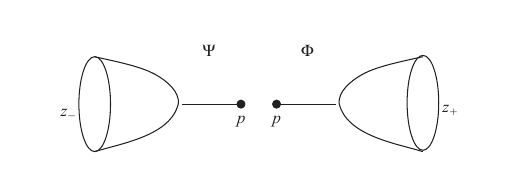
\includegraphics[width=.62\textwidth]{chapters/ch20-pants-product/figures/figure-20-1.png}
 \caption{PSS 映射 $\Psi$ 与 $\Phi$。}
 \label{fig:20-pss-maps}
\end{figure}

这里同样施加指标条件
\[
 \mu_{H_-}([z_-,w_-])=n-(\mu_{(-f)}(p)-2c_1(A_-)),
\]
使 $\mathcal M([z_-,w_-],p;A_-)$ 成为零维（可定向）流形。同样的延拓映射论证说明
$\Psi$ 是链映射，故在同调上诱导同态。

\stfhIndex{I028}{Jueretuihua}{绝热退化（adiabatic degeneration）}
\subsection{\personFloer{}模空间的绝热退化}

本小节描述 (OhZ11b) 建立的主要绝热粘合结果，不深入高度非平凡的分析细节；完整
细节见原文。在 $U_\pm$ 上用给定解析坐标 $z=e^{2\pi(\tau+it)}$，固定函数
\begin{equation}
 \kappa^+(\tau)=\begin{cases}0,&|\tau|\leq1,\\1,&|\tau|\geq2,
 \end{cases}
 \label{eq:20-kappa-plus}
\end{equation}
并令 $\kappa^-(\tau)=\kappa^+(-\tau)$。置
$\kappa_\epsilon^+(\tau)=\kappa^+(\tau-R(\epsilon)+1)$、
$\kappa_\epsilon^-(\tau)=\kappa_\epsilon^+(-\tau)$。容易看出
\begin{equation}
 \kappa_\epsilon^+(\tau)=\begin{cases}
 1,&\tau\geq R(\epsilon)+1,\\0,&\tau\leq R(\epsilon),
 \end{cases}
 \qquad
 \kappa_\epsilon^-(\tau)=\begin{cases}
 1,&\tau\leq-R(\epsilon)-1,\\0,&\tau\geq-R(\epsilon).
 \end{cases}
 \label{eq:20-kappa-epsilon-pm}
\end{equation}
再把它们在坐标卡 $U_\pm$ 外延拓为零。选取 $R=R(\epsilon)$，使
\begin{equation}
 \epsilon R(\epsilon)\longrightarrow0\qquad(\epsilon\to0).
 \label{eq:20-epsilon-r-normalization}
\end{equation}
绝热退化论证中的归一化步骤将用到这一选取。

还取截断函数 $\kappa_\epsilon^0:\mathbb R\to[0,1]$，满足
\begin{equation}
 \kappa_\epsilon^0(\tau)=\begin{cases}
 1,&|\tau|\leq R(\epsilon)-1,\\0,&|\tau|\geq R(\epsilon),
 \end{cases}
 \label{eq:20-kappa-zero}
\end{equation}
以及
\begin{equation}
 |(\kappa_\epsilon^0)'(\tau)|\leq2
 \qquad\text{当 }R(\epsilon)-1\leq|\tau|\leq R(\epsilon).
 \label{eq:20-kappa-derivative}
\end{equation}
考虑偶对 $(K_\epsilon,J_\epsilon)$ 的单参数族，其圆柱端为
\[
 \operatorname{End}_\pm(K_\epsilon,J_\epsilon)=(H,J),
 \qquad R_0\leq R(\epsilon)<\infty,
\]
其中 $(H,J)$ 是给定的\termFloerRegular{}偶对，具体如下。定义
\begin{equation}
 J_\epsilon(\tau,t,x)=\begin{cases}
 J^{\kappa_\epsilon^+(\tau)}(t,x),&\tau\geq R(\epsilon),\\
 J_0(x),&|\tau|\leq R(\epsilon)-1,\\
 J^{\kappa_\epsilon^-(\tau)}(t,x),&\tau\leq-R(\epsilon),
 \end{cases}
 \label{eq:20-j-epsilon}
\end{equation}
\footnote{译者注：原书分段条件在
$R(\epsilon)-1<|\tau|<R(\epsilon)$ 留出未定义的过渡带，却紧接着断言该族光滑。
截断函数显然意在填充该带，但页内未给出唯一公式，故译文照录。}
由上述截断函数，这定义了 $M$ 上一个光滑的 $\mathbb R\times S^1$ 殆复结构族。
类似地，定义 $K_\epsilon:\mathbb R\times S^1\times M\to\mathbb R$ 为
\begin{equation}
 K_\epsilon(\tau,t,x)=\begin{cases}
 \kappa_\epsilon^+(\tau)H(t,x),&\tau\geq R(\epsilon),\\
 \kappa_\epsilon^0(\tau)\epsilon f(x),&|\tau|\leq R(\epsilon),\\
 \kappa_\epsilon^-(\tau)H(t,x),&\tau\leq-R(\epsilon).
 \end{cases}
 \label{eq:20-k-epsilon}
\end{equation}

\begin{remark}
\label{rem:20-choice-k-epsilon}
\begin{enumerate}[label=(\arabic*)]
\item 定义 $K_\epsilon$ 时，我们使用线性同伦 $s\mapsto sH$；它由给定哈密顿量
$H=H(t,x)$ \emph{典范}确定。对任意同伦 $\mathcal H:s\mapsto H(s)$ 也可类似定义，其中
$H(s)=H(s,t,x)$ 是满足 $H(0)=\epsilon f$、$H(1)=H$ 的二参数族。所得同调映射与
同伦选取无关。
\item 比较上述 $K_\epsilon$ 与 (PSS96, MSa04) 的选取：他们使用颈部区域上
$K_\epsilon\equiv0$ 的族；我们则在颈部放入小\personMorse{}函数 $\epsilon f$，并取
$\epsilon\to0$ 的绝热极限。若颈部 $K_\epsilon\equiv0$，则在 (PSS96, MSa04) 所述
粘合构造中，很难从极限恢复\personFloer{}流线随 $\epsilon\to0$ 退化成节点流线的过程。
另一方面，我们在极限节点处提供记住背景\personMorse{}函数的一阶喷注数据。
\end{enumerate}
\end{remark}

对给定截断函数 $\kappa=\{\kappa_+,\kappa_-\}$，使用这个单参数族 $(K_R,J_R)$，
考虑参数化模空间
\[
 \begin{aligned}
 \mathcal M^{\mathrm{para}}([z_-,w_-],[z_+,w_+];\{(K,J;\kappa)\})
 &=\bigcup_{0<\epsilon\leq\epsilon_0}\{\epsilon\}\times
 \mathcal M([z_-,w_-],[z_+,w_+];K_\epsilon,J_\epsilon).
 \end{aligned}
\]
也简记 $\mathcal M^{\mathrm{para}}=\bigcup_{0<\epsilon\leq\epsilon_0}\mathcal M^\epsilon$。
为研究同调上的 $\Psi\circ\Phi$，需要分析 $\mathcal M^{\mathrm{para}}$ 的紧化。

以下关键分析定理完成 (Pi94), (PSS96) 所述 PSS 映射同构性质所需的论证。

\begin{theorem}[{(OhZ11b) 的定理 10.19}]
\label{thm:20-adiabatic-gluing}
令 $(K_\epsilon,J_\epsilon)$ 为~\eqref{eq:20-k-epsilon} 中定义的\personFloer{}数据族，则：
\begin{enumerate}[label=(\arabic*)]
\item 在
$\mathcal M^{\mathrm{para}}_{(0;1,1)}([z_-,w_-],[z_+,w_+];\{(K_\epsilon,J_\epsilon)\})$
上存在一种拓扑，使粘合构造对充分小的 $\epsilon_0$ 定义真嵌入
\[
 \begin{aligned}
 \operatorname{Glue}:{}&(0,\epsilon_0)\times
 \mathcal M^{\mathrm{nodal}}_{(0;1,1)}
 ([z_-,w_-],[z_+,w_+];(H,J),(f,J_0))\\
 &\longrightarrow
 \mathcal M^{\mathrm{para}}_{(0;1,1)}
 ([z_-,w_-],[z_+,w_+];\{(K,J)\}).
 \end{aligned}
\]
\item 上述拓扑可紧化为
$\overline{\mathcal M}^{\mathrm{para}}_{(0;1,1)}$，且作为集合
\[
 \overline{\mathcal M}^{\mathrm{para}}_{(0;1,1)}
 =\bigcup_{0<\epsilon\leq\epsilon_0}\{\epsilon\}\times
 \mathcal M_{(0;1,1)}(K_\epsilon,J_\epsilon)
 \ \cup\ \mathcal M^{\mathrm{nodal}}_{(0;1,1)}((H,J),(f,J_0)).
\]
\item 嵌入 $\operatorname{Glue}$ 光滑延拓为 $[0,\epsilon_0)$ 上的嵌入
$\overline{\operatorname{Glue}}$，满足
\[
 \overline{\operatorname{Glue}}(u_+,u_-,u_0;0)=\operatorname{Glue}(u_+,u_-,u_0).
\]
\end{enumerate}
\end{theorem}

完整证明见 (OhZ11b)。

\begin{figure}[htbp]
 \centering
 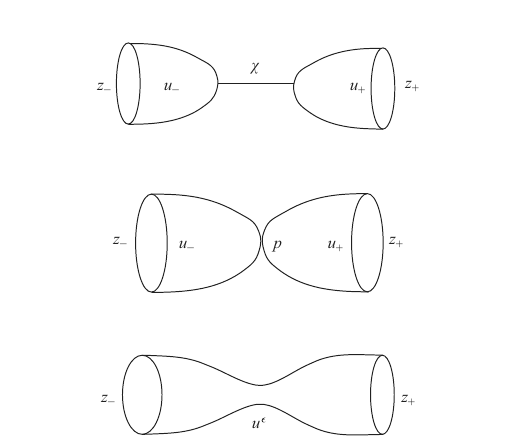
\includegraphics[width=.62\textwidth]{chapters/ch20-pants-product/figures/figure-20-2.png}
 \caption{PSS 方案。}
 \label{fig:20-pss-scheme}
\end{figure}

\subsection{证明的 PSS 方案}

\stfhIndex{I153}{Piwunixin-Salameng-Shiwaci}{皮乌尼欣--萨拉蒙--施瓦茨（Piunikhin--Salamon--Schwarz）}
本小节概述\personPiunikhin{}、\personSalamon{}和\personSchwarz{}对 PSS 映射同构性质的论证；它基于一个
形变，把复合映射
\[
 \Phi\circ\Psi:CF_*(H_+)\longrightarrow CF_*(H_+)
\]
与恒等映射之间建立链同伦。形变过程中涉及三类模空间（见图~\ref{fig:20-pss-scheme}）：
\footnote{译者注：原书此处称形变导向复合映射与恒等映射之间的“chain
isomorphism”，但随后构造的是链同伦并明确写出链同伦公式；译文据此写作“链同伦”。}
\begin{samepage}
\begin{enumerate}[label=(\arabic*)]
\item 圆盘--流--圆盘；
\item 节点\personFloer{}流线；
\item 链映射\personFloer{}流线。
\end{enumerate}
\end{samepage}

以下以 $\lambda\in[-1,1]$ 表示形变参数，使节点位形出现在 $\lambda=0$。只要
$\lambda>0$ 或 $\lambda<0$，形变所涉及的模空间类型相同，故标准论证分别在
$[-1,-\epsilon_0]$ 和 $[\epsilon_0,1]$ 上构造配边。要把配边延拓到整个区间，需要
用 $[-\epsilon_0,\epsilon_0]$ 上的配边连接二者。然而，模空间在 $\lambda=0$ 发生
“相变”，所以先验地只能期望得到\emph{分片光滑}配边；必须证明
$\mathcal M_0\subset\mathcal M^{\mathrm{para}}$ 的\emph{双领口定理}，才能实现 PSS 方案。
从 $-\epsilon_0$ 到 $0$ 的左单侧领口可由有限维构造得到（见 (OhZ11b) 第 9 节）；
$[0,\epsilon_0]$ 上右单侧领口的构造是非平凡的，它基于定理~\ref{thm:20-adiabatic-gluing}，
其证明使用 (OhZ11b) 的绝热退化方法。

应用定理~\ref{thm:20-adiabatic-gluing}，并逐字重复 (OhZ11b) 的论证（该论证又大体
沿用 (PSS96)），可证明下述 (PSS96) 中的同构性质。

\begin{theorem}
\label{thm:20-pss-one-sided-inverse}
令 $(-f;g)$ 为 $M$ 上\personMorse{}函数 $f$ 与度量 $g$ 的通有\personMorse{}--\personSmale{}偶对，
$H^{\mathrm{Morse}}(-f;g)$ 为其\personMorse{}同调。令 $(H,J)$ 为通有的含时周期哈密顿量
$H$ 与 $M$ 上相容殆复结构族 $J=\{J_t\}$。设 $\Psi,\Phi$ 为 (PSS96) 中的 PSS
映射。则存在同态
\[
 \Upsilon_{\mathrm{PSS}}:CF_*(H,J)\longrightarrow CF_{*+1}(H,J)
\]
满足
\begin{equation}
 \Phi\circ\Psi-\operatorname{id}
 =\partial_{(H,J)}\circ\Upsilon_{\mathrm{PSS}}
 -\Upsilon_{\mathrm{PSS}}\circ\partial^{\mathrm{Morse}}_{(-f,g)}.
 \label{eq:20-pss-chain-homotopy}
\end{equation}
\footnote{译者注：原书此式两项之间为减号；本节稍后的链同伦公式却使用加号。
这可能涉及作者的边界算子符号约定，也可能是排印不一致。此外，原书第二项使用
$\partial^{\mathrm{Morse}}_{(-f,g)}$，但 $\Upsilon_{\mathrm{PSS}}$ 的定义域和值域均为
$CF_*(H,J)$，故该复合在类型上也不成立；译文两处均照录。}
特别地，在同调上 $\Phi_*\circ\Psi_*=\operatorname{id}$。
\end{theorem}

这说明 $\Phi_*\circ\Psi_*=\operatorname{id}$。另一个恒等式
$\Psi_*\circ\Phi_*=\operatorname{id}$ 更容易证明；细节见 (OhZ11b) 第 9 节。

\begin{remark}
\label{rem:20-one-jet-datum}
\personFloer{}流线方程解模空间带中部\personMorse{}函数 $\epsilon f$ 的绝热退化，不仅产生 PSS 方案所用
的节点\personFloer{}流线，还产生带一阶喷注数据的节点\personFloer{}流线；该数据反映背景\personMorse{}函数 $f$ 的存在。这在 (OhZ11b) 的尺度依赖粘合中至关重要。
\end{remark}

\subsection{\texorpdfstring{$\Phi_*\circ\Psi_*=\operatorname{id}$}{Phi o Psi = id}：从\personFloer{}经\personMorse{}回到\personFloer{}}

考虑定义在 $\kappa\in[-\infty,1]$ 上的 PSS 形变。固定通有同伦
$(K^\kappa,J^\kappa)$，其中
$K^\kappa=K^\kappa(\tau,t,x)$、$J^\kappa=J^\kappa(\tau,t,x)$，它从
$(K^{\epsilon_0},J^{\epsilon_0})$ 连接到
$(K^1(\tau,t,x),J^1(\tau,t,x))=(H(t,x),J(t,x))$。
固定充分小的 $\epsilon_0>0$ 与充分大的 $\ell_0>0$，把形变分成四段：
\[
 \begin{array}{ll}
 (K^\kappa,J^\kappa),&\epsilon_0\leq\kappa\leq1,\\
 (K_\epsilon,J_\epsilon),&0<\kappa=\epsilon\leq\epsilon_0,\\
 (H^{\rho_-},J^{\rho_-})_{o_-}*(-f,g_{J_0};[-\ell,\ell])_{*_{o_+}}
 (H^{\rho_+},J^{\rho_+}),&-\ell_0\leq\ell<0,\\
 (H^{\rho_-},J^{\rho_-})_{o_-}*(-f,g_{J_0};[-\ell,\ell])_{*_{o_+}}
 (H^{\rho_+},J^{\rho_+}),&-\infty\leq\ell<-\ell_0.
 \end{array}
\]
这里 $(f,J_0;[-\ell,\ell])$ 表示形变
\[
 \ell\in(-\infty,0)\longmapsto(-f,g_{J_0};[-\ell,\ell]),
\]
其中 $f$ 是相对于度量 $g_{J_0}$ 的\personMorse{}函数，我们考虑其在区间
$[-\ell,\ell]$ 上的梯度流线。

以 $\mathcal M_\kappa^{\Psi\Phi}([z_-,w_-],[z_+,w_+])$ 表示对应参数 $\kappa$ 的
位形模空间，以参数化模空间表示整个形变：
\[
 \overline{\mathcal M}_{\Psi\Phi}^{\mathrm{para}}
 ([z_-,w_-],[z_+,w_+];f)
 =\bigcup_{\kappa\in[-1,\infty]}
 \mathcal M_\kappa^{\Psi\Phi}([z_-,w_-],[z_+,w_+]).
\]
\footnote{译者注：本小节开头把参数域写作 $[-\infty,1]$，此处却反向写作
$[-1,\infty]$；随后各段又使用负无穷端与上端 $1$，故两处不能同时成立。译文照录。}
由非退化假设和指标条件，除有限多个点外 $\mathcal M_\kappa^{\Psi\Phi}$ 为空；这些点
位于
\[
 \kappa\in(-\ell_0,-\ell_1)\cup(\epsilon_0,1).
\]
先验地，当 $\kappa\to0$ 时它们可能在 $[-\ell_1,\epsilon_0]$ 内聚集。但对应
$\kappa=0$ 的加强节点\personFloer{}流线模空间的一阶喷注横截性，以及
定理~\ref{thm:20-adiabatic-gluing} \emph{排除}了这种聚集。因此，若取 $\ell_1,\epsilon_0$
充分小，则对所有 $\kappa\in[-\ell_1,\epsilon_0]$ 有
\[
 \mathcal M_\kappa^{\Psi\Phi}([z_-,w_-],[z_+,w_+])=\varnothing.
\]
结合主要粘合紧性结果和定理~\ref{thm:20-adiabatic-gluing}，得到：

\begin{proposition}
\label{prop:20-phi-psi-compactification}
存在常数 $\ell_0,\ell_1,\epsilon_0,\epsilon_1$，使：
\begin{enumerate}[label=(\arabic*)]
\item 若 $\mu_H([z_-,w_-])-\mu_H([z_+,w_+])=-1$，则
$\overline{\mathcal M}_{\Psi\Phi}^{\mathrm{para}}([z_-,w_-],[z_+,w_+])$
是紧零维流形，并且当
$\kappa\in[-\infty,-\ell_0]\cup[-\ell_1,\epsilon_0]\cup[1-\epsilon_1,1]$
时 $\mathcal M_\kappa^{\Psi\Phi}=\varnothing$。
\item 若指标差为 $0$，则
$\overline{\mathcal M}_{\Psi\Phi}^{\mathrm{para}}([z_-,w_-],[z_+,w_+];f)$
是紧一维流形，其边界为
\[
 \begin{aligned}
 \partial\overline{\mathcal M}_{\Psi\Phi}^{\mathrm{para}}
 &=\mathcal M_{\kappa=1}([z_-,w_-],[z_+,w_+])
 \cup\mathcal M_{-\infty}([z_-,w_-],[z_+,w_+])\\
 &\quad\cup\bigcup_{[z,w]}
 \overline{\mathcal M}_{\Psi\Phi}^{\mathrm{para}}([z_-,w_-],[z,w])
 \#\mathcal M_{\kappa=1}([z,w],[z_+,w_+])\\
 &\quad\cup\bigcup_{[z,w]}
 \mathcal M_{\kappa=1}([z_-,w_-],[z,w])
 \#\overline{\mathcal M}_{\Psi\Phi}^{\mathrm{para}}([z,w],[z_+,w_+]),
 \end{aligned}
\]
第一、第二个并分别遍历满足相应指标差为 $-1$ 的 $[z,w]$。
\end{enumerate}
\end{proposition}

命题 (1) 可定义阶数为
$\#\overline{\mathcal M}_{\Psi\Phi}^{\mathrm{para}}([z_-,w_-],[z_+,w_+];f)$
的矩阵系数，从而定义映射
\[
 \Upsilon_{\mathrm{PSS}}^{\Psi\Phi}:CF_*(H)\to CF_{*+1}(H),
\]
其矩阵系数为
\[
 \langle\Upsilon_{\mathrm{PSS}}^{\Psi\Phi}([z_-,w_-]),[z_+,w_+]\rangle
 =\#\overline{\mathcal M}_{\Psi\Phi}^{\mathrm{para}}([z_-,w_-],[z_+,w_+];f).
\]
命题 (2) 对一维模空间边界的描述转化为
\[
 \Phi\circ\Psi-\operatorname{id}
 =\partial\circ\Upsilon_{\mathrm{PSS}}^{\Psi\Phi}
 +\Upsilon_{\mathrm{PSS}}^{\Psi\Phi}\circ\partial.
\]
这完成了同调上 $\Phi_*\circ\Psi_*=\operatorname{id}$ 的证明。

\subsection{\texorpdfstring{$\Psi_*\circ\Phi_*=\operatorname{id}$}{Psi o Phi = id}：从\personMorse{}经\personFloer{}回到\personMorse{}}

对每一对 $p,q\in\operatorname{Crit}f$，考虑参数化模空间
\[
 \overline{\mathcal M}_{\Phi\Psi}^{\mathrm{para}}(p,q)
 =\bigcup_{0\leq R\leq\infty}\mathcal M_R^{\Phi\Psi}(p,q).
\]
定义如下。对每个 $0<R<\infty$，先引入方程
\begin{equation}
 \overline\partial_{(K^R,J^R)}u=0
 \label{eq:20-r-dependent-cr}
\end{equation}
在 $\Sigma$ 上的有限能量解模空间
$\mathcal M_{(2;0,0)}(K^R,J^R)$。这里 $\Sigma$ 是带两个标记点
$\{o_-,o_+\}$ 的\personRiemann{}曲面，满足
$\Sigma\setminus\{o_\pm\}\cong\mathbb R\times S^1$。先以连通和定义\personRiemann{}曲面族 $(\Sigma,j_R)$：
\[
 (D^-,o_-)\cup C_R\cup(D^+,o_+),\qquad
 j_R=j_{D^-}\#j_{C_R}\#j_{D^+},
\]
其中 $C_R=[-R,R]\times S^1$，$j_{C_R}$ 是标准共形结构，$j_R$ 是
$D^-\cup C_R\cup D^+$ 上显然的粘合共形结构。以 $(\tau,t)$ 表示
$D^-\cup C_R\cup D^+\setminus\{o_-,o_+\}$ 上延拓 $C_R$ 标准坐标的共形坐标。

在这些坐标中固定截断函数族
\[
 \chi^R(\tau)=\begin{cases}
 1-\kappa^+(\tau-R),&\tau\geq0,\\
 1-\kappa^-(\tau+R),&\tau\leq0,
 \end{cases}
\]
其中 $1\leq R<\infty$；对 $0\leq R\leq1$ 令 $\chi^R=R\chi^1$。注意
$\chi^0\equiv0$，$\chi^R$ 具有紧支集，并且对任意给定紧子集，当 $R$ 充分大时
$\chi^R\equiv1$。因此，方程~\eqref{eq:20-r-dependent-cr} 在标记点 $o_\pm$ 附近化为
$\overline\partial_{J_0}u=0$。如前定义 $(K^R,J^R)$。

有两个评价映射
\[
 \operatorname{ev}_{o_\pm}:\mathcal M_{(2;0,0)}(K^R,J^R)\to M,
 \qquad\operatorname{ev}_{o_\pm}(u)=u(o_\pm).
\]
记
\[
 \begin{aligned}
 \widetilde{\mathcal M}^-(p;f)
 &=\{\chi:\mathbb R\to M\mid\dot\chi+\nabla(-f)(\chi)=0,
 \ \chi(-\infty)=p\},\\
\widetilde{\mathcal M}^+(q;f)
&=\{\chi:\mathbb R\to M\mid\dot\chi+\nabla(-f)(\chi)=0,
 \ \chi(+\infty)=q\},
\end{aligned}
\]
\footnote{译者注：原书把以上两处映射的类型写成“$\chi:\mathbb R\times M$”，没有
给出值域；由微分方程及端点条件可知应为 $\chi:\mathbb R\to M$，译文据此补正。}
并定义
\[
 \widetilde{\mathcal M}_1^-(p;-f)=\widetilde{\mathcal M}^-(p;-f)\times\mathbb R,
 \qquad
 \widetilde{\mathcal M}_1^+(q;-f)=\widetilde{\mathcal M}^+(q;-f)\times\mathbb R.
\]
$\tau_0\in\mathbb R$ 通过
$(\tau_0,(\chi,\tau))\mapsto(\chi(*-\tau_0),\tau+\tau_0)$ 自由作用，故商
\[
 \mathcal M_1^-(p;-f)=\widetilde{\mathcal M}_1^-(p;-f)/\mathbb R,
 \quad
 \mathcal M_1^+(q;-f)=\widetilde{\mathcal M}_1^+(q;-f)/\mathbb R
\]
\footnote{译者注：原书先以参数“$f$”定义 $\widetilde{\mathcal M}^{\pm}(\cdot;f)$，
但方程已使用 $\nabla(-f)$；紧接着又把同一对象代入参数“$-f$”定义
$\mathcal M_1^{\pm}(\cdot;-f)$。若逐字代入会反转梯度号，故此处存在记号不一致；
译文保留原书记号。}
分别是维数 $\mu_{\mathrm{Morse}}(p;f)$ 与
$2n-\mu_{\mathrm{Morse}}(q;f)$ 的光滑流形。其渐近评价映射
\[
 \operatorname{ev}_+:\mathcal M_1^+(q;-f)\to M,
 \qquad \operatorname{ev}_-:\mathcal M_1^-(p;-f)\to M
\]
的像分别与不稳定流形 $W^u(p;-f)$ 和稳定流形 $W^s(q;-f)$ 一一对应。
\footnote{译者注：原书按 $\operatorname{ev}_+$、$\operatorname{ev}_-$ 的顺序列出
定义域 $\mathcal M_1^+(q;-f)$、$\mathcal M_1^-(p;-f)$，却说其像“分别”为
$W^u(p;-f)$、$W^s(q;-f)$；变量和稳定/不稳定流形均与该顺序不匹配。译文照录。}

定义 $\mathcal M_R^{\Phi\Psi}(p,q;A)$ 为\termFiberProduct{}
\[
 \begin{aligned}
 \mathcal M_R^{\Phi\Psi}(p,q;A)
 &=\mathcal M_1^-(p;-f)_{\operatorname{ev}_-}
 \times_{\operatorname{ev}_{o_-}}\mathcal M_{(2;0,0)}(K^R,J^R;A)\\
 &\qquad{}_{\operatorname{ev}_{o_+}}
 \times_{\operatorname{ev}_+}\mathcal M_1^+(q;-f)\\
 &=\{((\chi_-,\tau_-),u,(\chi_+,\tau_+))\mid
 \chi_-(\tau_-)=u(o_-),\ \chi_+(\tau_+)=u(o_+)\},
 \end{aligned}
\]
并令
\[
 \overline{\mathcal M}^{\Phi\Psi,\mathrm{para}}(p,q;A)
 =\bigcup_{0\leq R\leq\infty}\mathcal M_R^{\Phi\Psi}(p,q;A).
\]
直接计算得到
\[
 \dim^{\mathrm{virt}}\mathcal M_R^{\Phi\Psi}(p,q;A)
 =\mu_{\mathrm{Morse}}(p)-\mu_{\mathrm{Morse}}(q)+2c_1(A).
\]

\begin{proposition}
\label{prop:20-psi-phi-compactification}
取通有偶对 $(f,J_0)$，并令 $0<\epsilon_1<R_1$。
\footnote{译者注：原书在本命题开头先令 $0<\epsilon_1<R_1$，但第 (1) 项又说“存在
某个 $\epsilon_1>0$ 和 $R_1>0$”；证明末还写成相反的 $R_1\leq\epsilon_1$。这些
量词和不等式彼此不容，译文逐处照录。}
\begin{enumerate}[label=(\arabic*)]
\item 若 $\mu_{\mathrm{Morse}}(p)-\mu_{\mathrm{Morse}}(q)+2c_1(A)=-1$，
则存在某个 $\epsilon_1>0$ 与 $R_1>0$，使
$\overline{\mathcal M}^{\Phi\Psi,\mathrm{para}}(p,q;A)$ 是紧零维流形，并且当
$0\leq R\leq\epsilon_1$ 或 $R\geq R_1$ 时
$\mathcal M_R^{\Phi\Psi}(p,q;A)=\varnothing$。
\item 若上述指标为 $0$，则
$\overline{\mathcal M}^{\Phi\Psi,\mathrm{para}}(p,q;A)$ 是紧一维流形，其边界为
\[
 \partial\overline{\mathcal M}^{\Phi\Psi,\mathrm{para}}(p,q;A)
 =\mathcal M_0^{\Phi\Psi}(p,q;A)\cup\mathcal M_\infty^{\Phi\Psi}(p,q;A)
 \cup\bigcup_r\overline{\mathcal M}^{\Phi\Psi}(p,r;A),
\]
\footnote{译者注：原书边界式最后一项只含 $(p,r;A)$，使原先固定的输出 $q$ 消失；
若它描述\personMorse{}破裂，通常还应出现从 $r$ 到 $q$ 的因子。页内资料不足以唯一补全，
译文照录。}
其中最后的并遍历满足
$\mu_{\mathrm{Morse}}(p)-\mu_{\mathrm{Morse}}(r)+2c_1(A)=-1$ 的
$r\in\operatorname{Crit}(-f)$。
\end{enumerate}
\end{proposition}

\begin{proof}
当 $R=0$ 时，方程~\eqref{eq:20-r-dependent-cr} 化为
$\overline\partial_{J_0}u=0$。因为
$\mu_{\mathrm{Morse}}(p)-\mu_{\mathrm{Morse}}(q)+2c_1(A)=-1$ 是
$\mathcal M_0^{\Phi\Psi}(p,q;A)$ 的虚维数，对通有 $(f,J_0)$ 该空间必为空。这里强调，
此模空间只依赖 $(f,J_0)$，故通有性论证可与参数 $R$ 无关地应用。因此当
$R_1\leq\epsilon_1$ 且 $\epsilon_1>0$ 充分小时，同样成立。证明完毕。第 (2) 项留给
读者。
\end{proof}

由 (1) 定义链同伦映射
\[
 \Upsilon_{\mathrm{PSS}}^{\Phi\Psi}:
 CM_*(-f,g_{J_0};\Lambda_\omega)\to CM_{*+1}(-f,g_{J_0};\Lambda_\omega),
\]
其矩阵元为
\[
 \langle\Upsilon_{\mathrm{PSS}}^{\Phi\Psi}(p),q\#(-A)\rangle
 =\sum_{(r,A)}\#\left(\bigcup_r
 \overline{\mathcal M}^{\Phi\Psi,\mathrm{para}}(p,r;A)\right).
\]
\footnote{译者注：原书左端固定 $q$，右端却对 $(r,A)$ 求和又在括号内再对 $r$ 取并，
同时复用 $A$；该矩阵元的下标无法由页内资料唯一重构，译文照录。}

\begin{lemma}
\label{lem:20-zero-end-dimension}
设 $\mu_{\mathrm{Morse}}(p)-\mu_{\mathrm{Morse}}(q)+2c_1(A)=0$。若 $A\neq0$，则除非
$\mathcal M_0^{\Phi\Psi}(p,q;A)=\varnothing$，否则
\[
 \dim\mathcal M_0^{\Phi\Psi}(p,q;A)\geq2.
\]
当 $A=0$ 时，除非 $p=q$，否则
\[
 \dim\mathcal M_0^{\Phi\Psi}(p,q;A)\geq1.
\]
\end{lemma}

\begin{proof}
若 $A\neq0$，则 $(u;o_-,o_+)\in\mathcal M_{(2;0,0)}(K^R,J^R)$ 中的 $u$ 非常值。
定义域 $(\Sigma;o_-,o_+)$ 的共形自同构产生至少实二维族，与指标假设矛盾（半正
情形见 (Fl89b), (FHS95)，一般情形见 (FOn99), (LT98)）。

若 $A=0$，任何 $J_0$-全纯球面都为常值，相应位形
$(\chi_-,\text{常值},\chi_+)$ 因而成为完整梯度流线
$\chi=\chi_-\#\chi_+$。除非 $\chi$ 为常值（即 $p=q$），否则 $\mathbb R$-平移产生
至少一维族，再次与指标假设矛盾。
\end{proof}

现在可完成恒等式
\begin{equation}
 \Psi\circ\Phi-\operatorname{id}
 =\Upsilon_{\mathrm{PSS}}^{\Phi\Psi}\partial^{\mathrm{Morse}}_{(-f,g_{J_0})}
 +\partial^{\mathrm{Morse}}_{(-f,g_{J_0})}\Upsilon_{\mathrm{PSS}}^{\Phi\Psi}
 \label{eq:20-psi-phi-chain-homotopy}
\end{equation}
的证明。先验地，命题~\ref{prop:20-psi-phi-compactification} 只给出
\[
 \sum_{q,A}\langle(\Psi\circ\Phi-\operatorname{id})(p),q\#(-A)\rangle
 =\sum_{q,A}\left\langle
 \Upsilon_{\mathrm{PSS}}^{\Phi\Psi}\partial^{\mathrm{Morse}}_{(-f,g_{J_0})}(p)
 +\partial^{\mathrm{Morse}}_{(-f,g_{J_0})}\Upsilon_{\mathrm{PSS}}^{\Phi\Psi}(p),
 q\#(-A)\right\rangle.
\]
但上述引理蕴含
\[
 \langle(p),q\#(-A)\rangle=0,
\]
除非 $A=0$ 且 $p=q$。这便证明了~\eqref{eq:20-psi-phi-chain-homotopy}。

\stfhIndex{I092}{Fuluobeiniwusipeidui}{弗罗贝尼乌斯配对（Frobenius pairing）}
\section{\personFrobenius{}配对与对偶性}
\label{sec:frobenius-pairing-duality}

回忆~\eqref{eq:20-flat-qh}、\eqref{eq:20-sharp-qh} 中给出的同构
$\flat:QH^*(M)\to QH_*(M)$ 及其逆
$\sharp:QH_*(M)\to QH^*(M)$。仍分别以 $a^\flat,b^\sharp$ 表示这些映射下的像。

\begin{definition}[\personFrobenius{}配对]
\label{def:20-frobenius-pairing}
定义非退化配对
\begin{equation}
 \Delta=\langle\cdot,\cdot\rangle:
 QH^k(M)\otimes QH^{n-k}(M)\longrightarrow\Lambda_\omega^{(0)}
 \label{eq:20-frobenius-pairing}
\end{equation}
为
\begin{equation}
 \left\langle\sum_Aa_Aq^A,\sum_Bb_Bq^B\right\rangle
 =\sum_{C;\,c_1(C)=0}\left(\sum_A(a_A,b_{C-A})\right)q^C,
 \label{eq:20-frobenius-coefficients}
\end{equation}
其中 $(a_A,b_B)$ 是 $H^k(M,\mathbb Q)$ 与 $H_k(M,\mathbb Q)$ 之间的典范\personPoincare{}配对：
\[
 (a_A,b_B)=a_A\cap PD(b_B).
\]
\footnote{译者注：原书把第二因子的次数印作 $n-k$，而本书以 $\dim M=2n$，且本段
随即把 $H^k$ 与 $H_k$ 配对；通常的上同调\personPoincare{}配对应涉及 $2n-k$。原书在
命题 20.4.4 又重复 $n-k$，故译文照录并登记此疑点。}
由 $QH^*(M)$ 定义中的有限性条件，式~\eqref{eq:20-frobenius-coefficients} 的和总是
有限的，因而定义良好。
\end{definition}

\begin{proposition}
\label{prop:20-frobenius-cup}
以 $[M]$ 表示基本类，以 $1=PD[M]$ 表示 $QH^*(M)$ 的单位元。则
\[
 \langle a,b\rangle=(a\cup_Qb)\cap[M]=\langle(a\cup_Qb),1\rangle.
\]
\end{proposition}

\begin{proof}
只需对上同调类 $a,b\in H^*(M)$ 证明第一个等式。这时左端就是经典\personPoincare{}对偶配对
\[
 (a_A,b_{C-A})=a_A\cap PD(b_{C-A})=(a_A\cup b_{C-A})\cap[M].
\]
现计算右端。以闭链 $P_1,P_2$ 代表 $PD(a),PD(b)$。依定义，
$(a\cup_Qb)\cap[M]$ 位于 $H_0(M;\Lambda_\omega)\cong\Lambda_\omega$，由
\[
 \sum_{\alpha\in\pi_2(M)}
 \mathcal M_3(J_0;\alpha)_{(\operatorname{ev}_1,\operatorname{ev}_2,
 \operatorname{ev}_0)}\times(P_1\times P_2\times M)
 T^{\omega(\alpha)}e^{c_1(\alpha)}
\]
给出，其中 $c_1(\alpha)=0$，故
$(a\cup_Qb)\cap[M]\in\Lambda_\omega^{(0)}\subset\Lambda_\omega$。

另一方面，\termFiberProduct{}
$\mathcal M_3(J_0;\alpha)_{(\operatorname{ev}_1,\operatorname{ev}_2,
\operatorname{ev}_0)}\times(P_1\times P_2\times M)$ 定义一个包含在
$C_0(M;\mathbb Q)$ 中的闭链，故维数必须为零。这只有在 $\alpha=0$ 时才可能；
于是 $\mathcal M_3(J_0;\alpha)$ 的所有元素都是常值映射，否则模空间的维数必须至少
有两个实维数，对应第零个标记点 $z_0$ 的变化。注意，由于 $M$ 是整个空间，对
$z_0$ 没有限制，因此可自由移动 $z_0$ 而不影响映射，也不影响在标记点 $z_1,z_2$
处分别与 $P_1,P_2$ 的给定相交。这证明上述\termFiberProduct{}恰好化为经典帽积
$(a\cup_Qb)\cap[M]=(a,b)$。
\end{proof}

定义 $\mathbb Q$-双线性配对 $\Pi$：
\begin{equation}
 \Pi(a,b)=\pi_0\circ\Delta(a,b)=\pi_0(\langle a\cdot b,1\rangle),
 \label{eq:20-rational-pairing}
\end{equation}
其中 $\pi_0:\Lambda_{0,\omega}\to\mathbb Q$ 是显然的投影，
$\pi_0(\sum_Aa_Aq^A)=a_{A=0}$。

\begin{remark}
\label{rem:20-continuous-dual}
即使作为 $\mathbb Q$-向量空间，$QH_*(M)$ 的对偶向量空间 $(QH_*(M))^*$ 也\emph{不同构}于
标准量子上同调 $QH^*(M)$。上述配对实际诱导单射
\[
 QH^*(M)\lhook\joinrel\longrightarrow(QH_*(M))^*,
\]
其像位于 $QH_*(M)$ 上的\emph{连续}线性泛函集合中；这里连续性相对于
式~\eqref{eq:20-downward-valuation} 的\termValuation{} $v$ 所诱导的拓扑而言。
\end{remark}

\begin{proposition}
\label{prop:20-pi-nondegenerate}
$\Pi$ 非退化。换言之，若对所有 $b\in QH^{n-k}(M)$ 都有 $\Pi(a,b)=0$，则 $a=0$。
\end{proposition}

\begin{proof}
若 $\Pi(a,b)=0$，则 $\pi_0(\Delta(a,b))=0$，故
\[
 \sum_{C;\,c_1(C)=\omega(C)=0}\sum_A(a_A,b_{C-A})=0.
\]
但 $c_1(C)=\omega(C)=0$ 蕴含 $C=0$ 于 $\Gamma$，因此对所有
$b_{-A}\in H^{n-k}(M)$ 都有 $\sum_{A\in\Gamma}(a_A,b_{-A})=0$。若
$a\in QH^k(M)$，取 $b=a_{-A}q^{-A}$，其中 $a_{-A}\in QH^{n-k}(M)$，便证明
对所有 $A\in\Gamma$ 都有 $a_A=0$，故 $a=0$。
\footnote{译者注：原书直接取 $b=a_{-A}q^{-A}$，却未说明为何系数 $a_{-A}$ 同时
属于互补次数，亦未取与 $a_A$ 配对非零的\personPoincare{}对偶元素；此处类型与非退化性
论证均有缺口。译文照录。}
\end{proof}

在第 22.5.1 小节中，我们将把 $QH^*(M)$ 看成小\personMorse{}函数的\personFloer{}上同调，利用
$QH^*(M)$ 与 $HF_*(H)$ 之间的自然同构，进一步研究\personFrobenius{}配对
\eqref{eq:20-frobenius-pairing}、\personFloer{}复形配对 (19.7.49) 以及二者的关系。

